\documentclass[czech,bachelor,dept470,male]{diploma}
\usepackage[autostyle=true,czech=quotes]{csquotes}
\usepackage{enumitem,amsfonts,amssymb,amsmath}
\usepackage[backend=biber, style=iso-numeric, alldates=iso]{biblatex}
\usepackage[a-1b]{pdfx}
\ThesisAuthor{Christian Krutsche}
\CzechThesisTitle{Nestandardní číselné soustavy}
\EnglishThesisTitle{Non-Standard Numeral Systems}
\SubmissionDate{14. května 2020}
\Thanks{Děkuji RNDr. Pavlu Jahodovi, Ph.D. za odborné vedení práce, věcné připomínky, užitečné rady a vstřícnost při konzultacích. Taky za věnovaný čas během psaní bakalářské práce.}
\ThesisAssignmentImagePath{data/assignment}
\AuthorDeclarationImageFile{data/authorDeclaration}
\CzechAbstract{Cílem této práce je prozkoumat různé nestandardní možnosti reprezentace čísel. Každý zná desítkovou soustavu ( ne nutně pod tímto označením ).\newline Poměrně známé jsou i soustavy, které se používají v praxi
\begin{itemize}
\item v každém technickém oboru - dvojková a šestnáctková 
\item při práci s časem, úhly - šedesátková
\end{itemize}
Kromě těchto standardních soustav, kterýchž základ tvoří posloupnost mocnin určitého\newline přirozeného čísla, můžeme jako základ soustavy definovat jinou posloupnost.\newline Prozkoumáme 4 číselné soustavy a u každé si řekneme jaký je její definiční obor,\newline jakým způsobem do této soustavy čísla převádíme, jestli se dá sčítat a násobit, případně jak takové operace provádíme.}
\CzechKeywords{číselná soustava, negabinární číselná soustava, komplexní číselná soustava, faktoriálová číselná soustava, Fibonacciho kódování}
\EnglishAbstract{The goal of this thesis is to explore various non-standard possibilities of representing numbers. The decimal number system is universally well known ( not necessarily under this label ).\newline Other common number systems that are used in practice are
\begin{itemize}
\item in technical fields - binary and hexadecimal
\item when working with time or angles - sexagesimal
\end{itemize}
Apart from standard systems (such as those mentioned above ), the base of which is a sequence of powers of a natural number, we can also use different sequences as base. We will examine 4 non-standard numeral systems and their characteristics. Such characteristics will include determining the domain of a system, the steps to achieve conversion, whether it is possible to add and multiply in the given numeral system, and if so, then how.}
\EnglishKeywords{numeral system, negabinary numeral system, complex-base system, factorial number system, Fibonacci coding}
\AddAcronym{$\mathbb{N}$}{Množina přirozených čísel}
\AddAcronym{$\mathbb{N}_0$}{Množina nezáporných celých čísel}
\AddAcronym{$\mathbb{Z}$}{Množina celých čísel}
\AddAcronym{$\mathbb{Z}[i]$}{Množina gaussových celých čísel}
\AddAcronym{$\left\lceil z\right\rceil$}{Horní celá část čísla $z$}
\AddAcronym{$\left\lfloor z\right\rfloor$}{Dolní celá část čísla $z$}
\AddAcronym{$\{a_i\}_{i=0}^\infty$}{Nekonečná posloupnost čísel}
\AddAcronym{$\varphi$}{Relace definující číselnou soustavu}
\AddAcronym{$|z|$}{Absolutní hodnota čísla $z$}
\AddAcronym{$N(z)$}{Norma čísla $z$}
\addbibresource{citation.bib}
\newcommand{\poslbeta}{\{\beta_i\}_{i=1}^{\infty}}
\newcommand{\poslalpha}{\{\alpha_i\}_{i=0}^{\infty}}
\newcommand{\posla}{\{a_i\}_{i=0}^{\infty}}
\newcommand{\poslb}{\{b_i\}_{i=1}^{\infty}}
\begin{document}
\MakeTitlePages
\section{Úvod}
Pojem číselná soustava je jistě znám každému, kdo studuje technickou školu. Jedná se o\newline systém, který nám umožňuje změnit množinu znaků, kterými reprezentujeme číslo.\newline Jak logika napovídá, čím více použitelných znaků pro reprezentaci máme, tím kratší bude\newline výsledná reprezentace (posloupnost znaků určující reprezentované číslo). Zprvu si definujeme co přesně číselná soustava je a jaké má vlastnosti, abychom se této definice mohli po zbytek práce držet. Následně se podíváme na 4 různé číselné soustavy. V každé kapitole, která se zabývá\newline soustavou bude nejdůležitější důkaz definičního oboru, který nám zajistí, že tímto způsobem\newline můžeme reprezentovat libovolné číslo z nějaké množiny. Jistě by se nikomu nelíbila\newline číselná soustava, která umožňuje reprezentovat jen konečný počet čísel, proto se budeme snažit, aby definičním oborem byla nekonečná množina. Kromě důkazu definičního oboru si popíšeme algoritmus, kterým budeme schopni převést číslo na reprezentaci v číselné soustavě.\newline A v neposlední řadě budeme experimentovat s myšlenkou, zda se dají reprezentace čísel v číselné soustavě sčítat, případně násobit. Jestliže dvě libovolná čísla půjdou sečíst a hodnota výsledku se bude opravdu rovnat součtu dvou čísel (což vlastně znamená, že číselná soustava jako zobrazení je homomorfní pro operaci sčítání), pak si taky ukážeme jak toho docílit. Stejnou úvahu provedeme ohledně operace násobení. Na konci každé kapitoly budeme uvažovat nad tím, zda by se tato soustava dala využít v nějakém reálném případě.\newpage
\subsection{Definice}
Připomeňme, že libovolnou podmnožinu $\varphi$ kartézského součinu $A \times B$ nazýváme binární relací (dále jen relací) mezi prvky z množiny $A$ a prvky z množiny $B$. Binární dvojici $(a,b)\in \varphi$ budeme značit $\varphi(a) = b$ a $\varphi \subseteq A \times B$ budeme značit $\varphi : A \rightarrow B$, tak jak je to obvyklé u zobrazení,\newline jež jsou speciálními případy relací.
\newline Následující definici jsme převzali z materiálu pro výuku matematické analýzy \cite{maUniverse}.
\begin{definition}
	Posloupností na množině M rozumíme každou funkci, jejímž definičním oborem je množina $\mathbb{N}$. Posloupnost, která každému $n \in \mathbb{N}$ přiřazuje číslo $a_n \in M$ budeme zapisovat některým z následujících způsobů:
	\begin{itemize}
		\item $a_0, a_1, a_2, a_3,\dots$
		\item $(a_n)$
		\item $\{a_n\}_{n=0}^{\infty}$
	\end{itemize}
\end{definition}
\begin{definition}\label{d2} \textbf{(Číselná soustava na tělese)}
	Nechť $(A,+,\cdot)$ je těleso; $\poslalpha$ a $\poslbeta$ jsou posloupnosti na množině $A$, $C\subseteq A$ a $B$ je množina všech posloupností prvků z $C$.
	\newline\textbf{Číselnou soustavou na tělese $(A,+,\cdot)$} o základu $\poslalpha$ a $\poslbeta$ s ciframi z $C$ nazveme libovolnou relaci $\varphi : A \rightarrow B\times B$, kde $\varphi(x)=\left(\{a_{i}\}_{i=0}^{\infty},\{b_{i}\}_{i=1}^{\infty}\right)$, právě když
	$$x = \sum_{i=0}^{\infty} a_{i}\alpha_{i} + \sum_{i=1}^{\infty} b_{i}\beta_{i}$$
	Množinu $C$ označujeme jako \textbf{množinu cifer} číselné soustavy $\varphi$. Budeme používat značení $\varphi(x) = \left(\{a_{i}\}_{i=0}^{\infty},\{b_{i}\}_{i=1}^{\infty}\right) = (\dots a_2,a_1,a_0;b_1, b_2, b_3, \dots)_{\varphi}$ a pokud nebude možno dojít k omylu, pak také $(\dots a_2,a_1,a_0;b_1, b_2, b_3, \dots)_{\varphi} = (\dots a_2,a_1,a_0;b_1, b_2, b_3, \dots) = (\dots a_2a_1a_0,b_1 b_2 b_3 \dots)$
\end{definition}
Všimněme si, že nevyžadujeme, aby $\varphi$ bylo zobrazení. Číselná soustava nemusí vyjadřovat každý prvek z $A$ a ty prvky z $A$, které jsou v relaci $\varphi$, nemusí být vyjádřeny jediným způsobem. Uvažujme například obvyklou desítkovou číselnou soustavu na tělese reálných čísel.\newline Jde o číselnou soustavu, kde $C = \{0, 1, 2, \dots, 9\}$ a základem jsou konstantní posloupnosti\newline $\poslalpha = \{10^i\}_{i = 0}^{\infty}$ a $\poslbeta = \{\frac{1}{10^i}\}_{i = 1}^{\infty}$
\newpage
\begin{enumerate}
	\item[I.] Vyjadřujeme jen nezáporná čísla, např. číslo $x = 1\cdot10^2 + 2\cdot10^1 + 3\cdot10^0 \Rightarrow \varphi(x) = (\dots123,000\dots)$, ale $\varphi(-x)$ neexistuje. Pomocí cifer z $C=\{0,\dots,9\}$ při základu $\{10^i\}_{i=0}^{\infty}$ nelze vyjádřit záporné číslo.
	\item[II.] ($\lfloor x\rfloor$ je celočíselná část reálného čísla $x$)
	      $$\varphi(1) = \left( \left\{ \left\lfloor\frac{1}{i+1} \right\rfloor \right\}_{i = 0}^{\infty} , \left\{ 0 \right\}_{i = 0}^{\infty} \right) = \left(\dots 001,000 \dots \right)$$
	      ale také
	      $$\varphi(1) = \left( \left\{ 0 \right\}_{i = 0}^{\infty} , \left\{ 9 \right\}_{i = 0}^{\infty} \right) = \left(\dots 000,999 \dots \right)$$
\end{enumerate}
Analogicky jako na tělese definujeme číselnou soustavu na okruhu.
\begin{definition}\label{d3} \textbf{(Číselná soustava na okruhu)}
	Nechť $(A,+,\cdot)$ je okruh, $\poslalpha$ je posloupnost prvků z $A$; $C\subseteq A$ a $B$ je množina všech posloupností prvků z $C$.
	\newline\textbf{Číselnou soustavou na okruhu $(A,+,\cdot)$} o základu $\poslalpha$ s ciframi z $C$ nazveme libovolnou relaci $\varphi : A \rightarrow B$, kde $\varphi(x)= \{a_{i}\}_{i=0}^{\infty}$, právě když
	$$x = \sum_{i=0}^{\infty} a_{i}\alpha_{i}$$
	Množinu $C$ označujeme jako \textbf{množinu cifer} číselné soustavy $\varphi$. Budeme používat značení $\varphi(x) = \{a_{i}\}_{i=0}^{\infty} = (\dots a_2,a_1,a_0)_{\varphi}$ a pokud nebude možno dojít k omylu,\newline pak také $(\dots a_2,a_1,a_0)_{\varphi} = (\dots a_2,a_1,a_0) = \dots a_2a_1a_0$
\end{definition}
\begin{remark}
	V Definici \ref{d2} a Definici \ref{d3} předpokládáme, že na tělese, respektive okruhu $(A,+,\cdot)$ jsou definovány nekonečné součty
\end{remark}
\begin{remark}
	Všimněme si, že číselná soustava $\varphi$, ať již na tělese, nebo na okruhu, splňuje:
	$$\varphi (x_1) = \varphi(x_2) \Rightarrow x_1 = x_2.$$
	Proto, je-li $\varphi$ zobrazení, je injektivní.
	Dále můžeme tvrdit, že hodnota $\varphi(x)$ ( i v případě, že $\varphi(x)$ není zobrazení ) jednoznačně určuje svůj vzor $x$. Jak jsme viděli výše, $x$ nemusí ale jednoznačně určovat svůj obraz $\varphi(x)$.
\end{remark}
\begin{definition}
	Jestliže pro číselnou soustavu $\varphi$ na tělese $(A,+,\cdot)$ platí, že $\varphi$ je zobrazení,\newline pak tuto soustavu nazveme \textbf{jednoznačnou číselnou soustavou na tělese $(A,+,\cdot)$}. Analogicky, jestliže pro číselnou soustavu $\varphi$ na okruhu $(A,+,\cdot)$ platí, že $\varphi$ je zobrazení, pak tuto soustavu nazveme \textbf{jednoznačnou číselnou soustavou na okruhu $(A,+,\cdot)$}
\end{definition}
Jednoznačnou číselnou soustavou na tělese (respektive okruhu), tedy nazveme každou číselnou soustavu v níž dokážeme vyjádřit libovolný prvek tělesa (okruhu) nejvýše jedním způsobem.
\begin{agreement}\label{u1}
	\begin{itemize}
		\item[]
		\item Nechť $\poslalpha$ a $\poslbeta$ jsou posloupnosti, které jsou základem číselné soustavy na tělese $(A,+,\cdot)$. Jestliže $\exists n \in A$, pro které platí:
		      $$ (\forall i \in \mathbb{N} : \alpha_i = n^i,\beta_i = n^{-i}) \land (\alpha_{0} = 1)$$
		      pak číslo \textbf{n} také nazýváme základem této číselné soutavy (1 označuje neutrální prvek tělesa $(A,+,\cdot)$ vzhledem k násobení).
		\item Nechť $\varphi(x) = (\posla,\poslb)$ je číselná soustava na tělese o základu \textbf{n}.\newline Pokud má posloupnost $\posla$ od jistého $n_1\in\mathbb{N}$ pouze nulové členy\newline a posloupnost $\poslb$ od $n_2\in\mathbb{N}$ pouze nulové členy, budeme zapisovat:
		      $$\varphi(x) = (a_{n_1} \dots a_0,b_1, b_2,\dots)_n$$
		\item V případě základu $\textbf{n}=10$ píšeme pouze $\varphi(x) = a_{n_1} \dots a_0,b_1 \dots b_{n_2}$
		\item Nechť $\poslalpha$ je posloupnost, která je základem číselné soustavy na okruhu $(A,+,\cdot)$\newline s jedničkou. Jestliže $\exists n \in A$, pro které platí:
		      $$(\forall i \in \mathbb{N}_0 : \alpha_i = n^i)$$
		      pak prvek \textbf{n} také nazýváme základem této číselné soutavy\newline $( n^0=1$ je jedničkou v okruhu $(A,+,\cdot) )$
		\item Nechť $\varphi(x) = (\posla)$ je číselná soustava na okruhu o základu \textbf{n}.\newline Pokud má posloupnost $\posla$ od jistého $n_1\in\mathbb{N}$ pouze nulové členy, budeme zapisovat: $\varphi(x) = (a_{n_1} \dots a_0)_n$
		\item Pokud zmíníme, že číslo z je v relaci s posloupností $\posla$ pro číselnou soustavu na okruhu o základu $\{\alpha_i\}_{i=0}^\infty$, pak dle definice číselné soustavy na okruhu jistě platí $z = \sum_{i=0}^{\infty} a_{i}\alpha_{i}$
	\end{itemize}
\end{agreement}
\newpage
\subsection{Názorné příklady}
Pro lepší představu definice číselné soustavy si ji předveďme na příkladu
\begin{example}
	Uvažujme těleso reálných čísel $(\mathbb{R},+,\cdot)$. Tj. zvolili jsme $A = \mathbb{R}$. Obvyklý desetinný zápis reálných čísel je vlastně číselná soustava na tělese $(\mathbb{R},+,\cdot)$ o základu $\poslalpha=\{{10^i\}}_{i=0}^{\infty}$,\newline $\poslbeta=\{{10^{-i}\}}_{i=1}^{\infty}$ a C = $\{0,1,2,3,4,5,6,7,8,9\}$. Podle Úmluvy \ref{u1} můžeme říci,\newline že jde o číselnou soustavu na tělese o základu 10 a platí:
	$$\varphi(3\cdot10^2+2\cdot10^1+5\cdot10^0+6\cdot10^{-1})=(\posla,\poslb)$$kde
	$\posla=(5,2,3,0,0,\dots)$ a $\poslb = (6,0,0,\dots)$\newline Podle Úmluvy \ref{u1} můžeme psát $$\varphi(3\cdot10^2+2\cdot10^1+5\cdot10^0+6\cdot10^{-1})=325.6$$
	Označme $x=3\cdot10^2+2\cdot10^1+5\cdot10^0+6\cdot10^{-1}$\newline
	$\varphi(-x) = \varphi(-(3\cdot10^2+2\cdot10^1+5\cdot10^0+6\cdot10^{-1}))$ neexistuje, ale prvek $-x$ ovykle značíme $-x=-\varphi(x)=-325.6$, neboť obvykle nerozlišujeme mezi číslem a jeho ciferným zápisem,\newline to jest mezi $-x$ a $\varphi(-x)$.
\end{example}
\section{Negabinární číselná soustava}
\begin{definition}
	Negabinární číselná soustava je číselná soustava na okruhu $(\mathbb{Z},+,\cdot)$ o základu -2 s množinou cifer $C=\{0,1\}$
\end{definition}
Negabinární číselná soustava je tedy relace $\varphi$ mezi celými čísly a posloupnostmi jedniček a nul, kde $z \in \mathbb{Z}$ je v relaci s posloupností $\posla$ právě tehdy, když
$$z=\sum_{i=0}^{\infty}a_i\cdot(-2)^i$$
Zmiňuje se o ní D. Knuth \cite{pcProg}
Ciferným zápisem celého čísla v negabinární číselné soustavě je posloupnost čísel z množiny $C=\{0,1\}$. Fakt, že $\varphi(z) = \posla$, kde $a_i = 0$ pro $i > k$, budeme symbolicky zapisovat $\varphi(z) = (a_k\,\dots\, a_0)_{-2}$. Pokud nebude moci dojít k omylu, tento zápis ještě zjednodušíme na $z = (a_k\,\dots\, a_0)_{-2}$. Například $5 = (101)_{-2}$, neboť $5 = 1\cdot(-2)^2 + 0\cdot(-2)^1 + 1\cdot(-2)^0$\newline
Prozkoumáme základní vlastnosti této číselné soustavy. Nejprve ukážeme, že v negabinární\newline číselné soustavě dokážeme najít ciferný zápis pro libovolné celé číslo.
\begin{theorem}\label{negaDF}
	Pro každé $z \in \mathbb{Z}$ existuje $\posla$, $a_i\in \{0,1\}$ taková, že
	$z=\sum_{i=0}^{\infty}a_i\cdot(-2)^i$\newline To jest, $D(\varphi)=\mathbb{Z}$.
\end{theorem}
\begin{proof}
	Protože $(\mathbb{Z},+,\cdot)$ je euklidovský obor integrity, jistě existují čísla $z_i\in\mathbb{Z}, a_i\in\{0,1\}$ taková, že:
	\begin{equation}\label{NBe1}
		\begin{array}{rcl}
			z = z_0 & =      & z_1\cdot(-2) + a_0       \\
			        &        &                          \\
			z_1     & =      & z_2\cdot(-2) + a_1       \\
			        &        &                          \\
			z_2     & =      & z_3\cdot(-2) + a_2       \\
			        & \vdots &                          \\
			z_{k-1} & =      & z_{k}\cdot(-2) + a_{k-1} \\
			        & \vdots &                          \\
		\end{array}
	\end{equation}
	V případě, že $z_1=0$, je jasné, že $z = a_0 = a_0(-2)^0$, kde $a_0\in\{0,1\}$. Dokazované tvrzení v tomto případě platí. Co když ale $z_0 \neq 0$?
	Dokážeme, že pro dost velké $n$ je $z_{n+1} = 0$.\newline Z (\ref{NBe1}) je zřejmé, že pro libovolné $k \in \mathbb{N}$ platí
	\begin{equation}\label{NBe2}
		|z_k|=\left|\frac{z_{k-1}-a_{k-1}}{-2}\right|\leq \frac{|z_{k-1}|+1}{2} = \frac{|z_{k-1}|}{2} + \frac{1}{2}
	\end{equation}
	Z (\ref{NBe2}) plyne, že pro $(k-1) \in \mathbb{N}$ také platí
	\begin{equation}\label{NBe3}
		|z_{k-1}|=\left|\frac{z_{k-2}-a_{k-2}}{-2}\right|\leq \frac{|z_{k-2}|}{2} + \frac{1}{2}.
	\end{equation}
	Aplikací odhadu (\ref{NBe3}) v (\ref{NBe2}) obdržíme
	\begin{equation*}\label{NBe4}
		|z_k| \leq \frac{|z_{k-1}|}{2} + \frac{1}{2} \leq \frac{|z_{k-2}|}{2^2} + \frac{1}{2} + \frac{1}{2^2}
	\end{equation*}
	Analogicky můžeme pokračovat a zjistíme, že pro libovolné $k \in \mathbb{N}$ platí
	\begin{equation}\label{NBe5}
		|z_k| \leq \frac{|z_0|}{2^k}+\sum_{i=1}^{k}\left(\frac{1}{2}\right)^i = \frac{|z_0|}{2^k}+1-\left(\frac{1}{2}\right)^k
	\end{equation}
	Vzhledem k tomu, že $\lim\limits_{k\to\infty}\frac{|z_0|}{2^k}+1-\left(\frac{1}{2}\right)^k=1$, je zřejmé, že existuje $k_0 \in \mathbb{N}$ takové, že $|z_{k_0}| \leq 1,5$\newline To ale znamená, že $z_{k_0} \in \{-1, 0, 1\}$. Rozeberme jednotlivé případy.
	\begin{enumerate}
		\item[a)] Jestliže $z_{k_0} = 0$, pak také $z_{k_0+1} = 0$. Hledaným $n$ proto může být $n = k_0$
		\item[b)] Jestliže $z_{k_0} = 1$, pak $z_{k_0} = 1 = z_{k_0+1}\cdot(-2)+a_{k_0}$. Protože $a_{k_0} \in \{0,1\}$,
		      musí platit $z_{k_0+1}=0$. Hledaným $n$ proto může být $n = k_0$
		\item[c)] Jestliže $z_{k_0} = -1$, pak $z_{k_0} = -1 = z_{k_0+1}\cdot(-2)+a_{k_0}$. Protože $a_{k_0} \in
			      \{0,1\}$, musí platit $z_{k_0+1}=1$. To ale podle předchozího bodu znamená, že $z_{k_0+2}=0$. Hledaným $n$ proto může být $n = k_0 + 1$
	\end{enumerate}
	Dokázali jsme, že existuje $n \in \mathbb{N}$ takové, že $z_{n+1} = 0$. Z toho plyne, že $z_n = a_n$,\newline odtud $z_{n-1} = a_n\cdot(-2)^1 + a_{n-1}$, \dots, $z = z_0 = a_n\cdot(-2)^n + a_{n-1}\cdot(-2)^{n-1} + \cdots + a_0$.\newline Pokud zvolíme $a_i = 0$ pro $i > n$, pak $z=\sum_{i=0}^{\infty}a_i\cdot(-2)^i$
\end{proof}
Na základě úvah provedených ve výše uvedeném důkazu Věty \ref{negaDF} můžeme vyslovit následující tvrzení.
\begin{theorem}\label{NBv2}
	Pro každé $z \in \mathbb{Z}$ existuje konečná posloupnost $\{a_i\}_{i=0}^k$, $a_i \in \{0, 1\}$ taková, že
	$$
		z = \sum_{i=0}^{k}a_i(-2)^i
	$$
\end{theorem}
\begin{proof}
	Z důkazu Věty \ref{negaDF} okamžitě plyne, že prokaždé celé číslo existuje posloupnost $\posla$\newline s konečným počtem nenulových prvků splňující $z=\sum_{i=0}^{\infty}a_i(-2)^i$
\end{proof}
Vzniká otázka, zda může existovat posloupnost $\posla$ splňující $z=\sum_{i=0}^{\infty}a_i(-2)^i$\newline i s nekonečným počtem nenulových prvků? Jinak řečeno, existuje nějaké celé číslo $z$, které je v relaci $\varphi$ s nějakou nekonečnou posloupností? Odpověď je záporná. V negabinární soustavě můžeme každé celé číslo vyjádřit jen pomocí konečného počtu nenulových cifer.
\newpage
\begin{theorem}\label{NBv2.5}
	Nechť $z \in \mathbb{Z}$. Jestliže $z=\sum_{i=0}^{\infty}a_i(-2)^i$, pak posloupnost $\posla$ má konečný počet nenulových členů.
\end{theorem}

\begin{proof}
	Důkaz provedeme sporem. Předpokládejme, že číslo $z=\sum_{i=0}^{\infty}a_i(-2)^i$, kde posloupnost $\posla$ má nekonečně mnoho nenulových členů. Pak může nastat právě jeden ze tří případů:
	\begin{itemize}
		\item[$a)$]
		      Mezi sudými členy posloupnosti $\posla$ (máme na mysli ta $a_n$, kde $n$ je sudé) je nekonečně mnoho
		      těch, které mají hodnotu $1$ a existuje jen konečný počet nenulových lichých členů posloupnosti $\posla$.
		      Je zřejmé, že $z = \sum_{i=0}^{\infty}a_i(-2)^i = \infty$. To je spor s tím, že $z \in \mathbb{Z}$.
		\item[$b)$] Mezi lichými členy posloupnosti $\posla$ (máme na mysli ta $a_n$, kde $n$ je liché) je nekonečně mnoho
		      těch, které mají hodnotu $1$ a existuje jen konečný počet nenulových sudých členů posloupnosti $\posla$.
		      Je zřejmé, že $z = \sum_{i=0}^{\infty}a_i(-2)^i = -\infty$. To je spor s tím, že $z \in \mathbb{Z}$.

		\item[$c)$] Jak mezi lichými, tak mezi sudými členy posloupnosti $\posla$ je nekonečně mnoho těch s nenulovou
		      hodnotou.
		      Uvažujme $n_k$ sudé, takové, že $a_{n_k} = 1$. Označme částečný součet
		      $$S_{n_k} = \sum_{i=0}^{n_k}a_i(-2)^i$$
		      Můžeme odhadnout hodnotu $S_{n_k}$:
		      \begin{equation}\label{NBe6}
			      \begin{array}{rcl}
				      S_{n_k} & =    & (-2)^{n_k} + \sum_{i=0}^{n_k-1}a_i(-2)^i =           \\
				              &      &                                                      \\
				              & =    & 2^{n_k} + \sum_{i=0}^{n_k-1}a_i(-2)^i \geq           \\
				              &      &                                                      \\
				              & \geq & 2^{n_k} - \sum_{i=0}^{n_k-1}2^i =                    \\
				              &      &                                                      \\
				              & =    & \displaystyle{2^{n_k} - \frac{2^{n_k} - 1}{2-1} = 1} \\
				              &      &                                                      \\
			      \end{array}
		      \end{equation}

		      Nyní uvažujme $n_k$ liché, takové, že $a_{n_k} = 1$ a odhadněme hodnotu $S_{n_k}$:
		      \begin{equation}\label{NBe7}
			      \begin{array}{rcl}
				      S_{n_k} & =    & (-2)^{n_k} + \sum_{i=0}^{n_k-1}a_i(-2)^i =               \\
				              &      &                                                          \\
				              & =    & - 2^{n_k} + \sum_{i=0}^{n_k-1}a_i(-2)^i \leq             \\
				              &      &                                                          \\
				              & \leq & - 2^{n_k} + \sum_{i=0}^{n_k-1}2^i =                      \\
				              &      &                                                          \\
				              & =    & \displaystyle{ - 2^{n_k} + \frac{2^{n_k} - 1}{2-1} = -1} \\
				              &      &                                                          \\
			      \end{array}
		      \end{equation}
		      Z (\ref{NBe6}) plyne, že pro $n_k$ sudé, kde $a_{n_k} = 1$ (a takových je podle předpokladu nekonečně mnoho), platí $S_{n_k} \geq 1$. Zároveň z (\ref{NBe7}) plyne, že pro $n_k$ liché, kde $a_{n_k} = 1$ (a takových je podle předpokladu také nekonečně mnoho), platí $S_{n_k} \leq -1$. To by však znamenalo,\newline že suma $\sum_{i=0}^{\infty}a_i(-2)^i$ nekonverguje. Opět docházíme ke sporu.
	\end{itemize}
\end{proof}
Nakonec dokážeme, že každé celé číslo je možné v negabinární číselné soustavě vyjádřit jen jedním způsobem, to jest, existuje právě jeden jeho ciferný zápis.
\begin{theorem}\label{NBv3}
	Pro každé $z\in\mathbb{Z}$ existuje jediná posloupnost $\{a_i\}_{i=0}^\infty$, $a_i \in\{0,1\}$ taková,\newline že $z = \sum_{i=0}^{\infty}a_i(-2)^i$
\end{theorem}
\begin{proof}
	Nejprve dokážeme tvrzení věty pro $z = 0$. Věta \ref{negaDF} říká, že existuje posloupnost $\posla$, $a_i \in \{0, 1\}$ taková, že $ 0 = \sum_{i=0}^{\infty}a_i(-2)^i$.
	Věta \ref{NBv2.5} navíc tvrdí, že posloupnost $\posla$ nemůže mít nekonečný počet nenulových členů. Musí proto existovat $k \in \mathbb{N}$ takové, že $a_i = 0$ pro $i > k$. Odtud
	\begin{equation}\label{NBv3e1}
		0 = \sum_{i=0}^{k}a_i(-2)^i
	\end{equation}
	Předpokládejme, že $a_k = 1$. Stejně jako v důkazu Věty \ref{NBv2.5} využijeme odhad součtu (\ref{NBv3e1}). Nejprve pro $k$ liché :
	\begin{equation}\label{NBv3e2}
		\begin{array}{rcl}
			0 = \sum_{i=0}^{k}a_i(-2)^i & =    & 1\cdot(-2)^{k} + \sum_{i=0}^{k-1}a_i(-2)^i =        \\
			                            &      &                                                     \\
			                            & =    & - 2^{k} + \sum_{i=0}^{k-1}a_i(-2)^i \leq            \\
			                            &      &                                                     \\
			                            & \leq & - 2^{k} + \sum_{i=0}^{k-1}2^i =                     \\
			                            &      &                                                     \\
			                            & =    & \displaystyle{- 2^{k} + \frac{2^{k} - 1}{2-1} = -1} \\
			                            &      &                                                     \\
		\end{array}
	\end{equation}
	Dostáváme sporné tvrzení $0 \leq -1$. Analogicky pro $k$ sudé :
	\begin{equation}\label{NBv3e3}
		\begin{array}{rcl}
			0 = \sum_{i=0}^{k}a_i(-2)^i & =    & 1\cdot(-2)^{k} + \sum_{i=0}^{k-1}a_i(-2)^i =      \\
			                            &      &                                                   \\
			                            & =    & 2^{k} + \sum_{i=0}^{k-1}a_i(-2)^i \geq            \\
			                            &      &                                                   \\
			                            & \geq & 2^{k} - \sum_{i=0}^{k-1}2^i =                     \\
			                            &      &                                                   \\
			                            & =    & \displaystyle{ 2^{k} - \frac{2^{k} - 1}{2-1} = 1} \\
			                            &      &                                                   \\
		\end{array}
	\end{equation}
	Opět dostáváme sporné tvrzení. Proto $a_k = 0$. Vedoucím koeficientem se tak stává $a_{k-1}$.\newline Opakováním ůvahy zjistíme, že všechny koeficienty $a_i$ musí být rovny nule.\newline Znamená to, že pro $z = 0$ existuje jediná posloupnost $\{a_i\}_{i=0}^\infty$, $a_i \in\{0,1\}$ taková,\newline že $z = \sum_{i=0}^{\infty}a_i(-2)^i$. Jedná se o posloupnost, kde $\forall\,i\in \mathbb{N}\, :\, a_i = 0$.\newline
	Nyní předpokládejme, že existuje nenulové celé číslo $z \neq 0$, které je v relaci $\varphi$ s posloupností $\posla$ a také s posloupností $\poslb$.
	Z Věty \ref{NBv2.5} plyne, že jak poslosloupnost $\posla$,\newline tak posloupnost $\poslb$, má jen konečně mnoho nenulových členů.\newline Označme $k_1 = \max\{i \in \mathbb{N}\,:\, a_i = 1\}$, $k_2 = \max\{i \in \mathbb{N}\,:\, b_i = 1\}$ a $k = \max\{k_1, k_2\}$\newline (čísla $k_1$ a $k_2$ jistě existují, neboť $z$ je nenulové). Potom jistě platí:
	\begin{equation}\label{NBv3e4}
		z=\sum_{i=0}^{k}a_i(-2)^i = \sum_{i=0}^{k}b_i(-2)^i
	\end{equation}
	Z (\ref{NBv3e4}) plyne, že
	\begin{equation}
		0 = \sum_{i=0}^{k}(a_i - b_i)(-2)^i
	\end{equation}
	Jak jsme ale výše dokázali, musí pro každé $i \in \{0, \dots, k\}$ platit $a_i - b_i = 0$. To ovšem znamená, že $\posla = \poslb$
\end{proof}
\begin{consequence}
	Negabinární číselná soustava je jednoznačná číselná soustava na okruhu celých čísel.
\end{consequence}
\begin{proof}
	Z Věty \ref{NBv3} okamžitě plyne, že relace $\varphi$ je zobrazení.
\end{proof}
Výše uvedené poznatky můžeme shrnout. V negabinární číselné soustavě dokážeme vyjádřit libovolné celé číslo pomocí konečného ciferného zápisu a to jediným způsobem.
\begin{remark} Algoritmus pro hledání reprezentace čísla v negabinární číselné soustavě je založen na konstrukci popsané v důkazu Věty \ref{negaDF}:\newline
	\begin{enumerate}
		\item Nechť $z$ je číslo, které chceme reprezentovat, $z_0 = z$ a $i=0$ je počáteční hodnota algoritmu.
		\item Pro pro $i>0$ ze vztahu $z_i=z_{i+1}\cdot(-2)+a_i$ určíme čísla $z_{i+1}$ a $a_i$ tak, aby platilo
		      $a_i\in\{0,1\}$
		\item Algoritmus končí pro $i = n$, kde $z_{n+1} = 0$.
		\item Potom $\posla$, kde $a_i=0$ pro každé $i>n$, splňuje požadavek $z=
			      \sum_{i=0}^{\infty}a_i\cdot(-2)^i$
	\end{enumerate}
\end{remark}
\begin{example} Vyjádříme číslo $z = 13$ v negabinární číselné soustavě.
	$$
		\begin{array}{rcrclcl}
			z_i & = & z_{i+1} & \cdot & (-2) & + & a_i \\ \hline
			    &   &         &       &      &   &     \\
			13  & = & -6      & \cdot & (-2) & + & 1   \\
			    &   &         &       &      &   &     \\
			-6  & = & 3       & \cdot & (-2) & + & 0   \\
			    &   &         &       &      &   &     \\
			3   & = & -1      & \cdot & (-2) & + & 1   \\
			    &   &         &       &      &   &     \\
			-1  & = & 1       & \cdot & (-2) & + & 1   \\
			    &   &         &       &      &   &     \\
			1   & = & 0       & \cdot & (-2) & + & 1   \\
			    &   &         &       &      &   &     \\
		\end{array}
	$$
	A opravdu, $1\cdot(-2)^0 + 1 \cdot(-2)^2+1\cdot(-2)^3+1\cdot(-2)^4 = 1 + 4 - 8 + 16 = 13$. Můžeme proto psát $\varphi(13) = (11101)_{-2}$.
\end{example}
\subsection{Sčítání celých čísel v negabinární číselné soustavě}
Sčítání čísel v negabinární číselné soustavě můžeme provádět podle schématu popsaného v\newline následujících příkladech.
\begin{itemize}
	\item Zvolme $a = 9$ a $b = 19$.\newline Dle výše uvedeného algoritmu nalezneme ciferný zápis těchto celých čísel $9 = (11001)_{-2}$ a $19 = (10111)_{-2}$. Cifry zapíšeme pod sebe do tabulky a do řádku pod nimi naznačíme pomocí čárek, kolik má součet $a+b$ příslušných mocnin čísla $-2$:
	      \begin{equation}\label{NBprsoucT1}
		      \begin{tabular}{|c|c|c|c|c|c|}
			      \hline
			      1  & 1 & 0 & 0 & 1  & a   \\ \hline
			      1  & 0 & 1 & 1 & 1  & b   \\ \hline \hline
			      || & | & | & | & || & a+b \\
			      \hline
		      \end{tabular}
	      \end{equation}
	      Třetí řádek Tabulky \ref{NBprsoucT1} znázorňuje fakt, že $a + b = 2\cdot(-2)^4 + (-2)^3 + (-2)^2 + (-2)^1 + 2\cdot(-2)^0$
	      Tento řádek můžeme dále upravovat a to dle následujících pravidel.\newline Protože $(-2)^{k+1} + 2\cdot(-2)^k = 0$, můžeme nahradit:
	      \begin{equation}\label{NBprsoucT2}
		      \begin{tabular}{|c|c|c|}
			      \hline
			      | & || & a+b \\ \hline
			      0 & 0  & a+b \\
			      \hline
		      \end{tabular}
	      \end{equation}
	      Protože $ 2\cdot(-2)^k = - (-2)^{k+1} $, můžeme nahradit:
	      \begin{equation}\label{NBprsoucT3}
		      \begin{tabular}{|c|c|c|}
			      \hline
			      0  & || & a+b \\ \hline
			      -| & 0  & a+b \\
			      \hline
		      \end{tabular}
	      \end{equation}
	      Protože $ -(-2)^k = (-2 + 1) \cdot(-2)^{k} = (-2)^{k+1} + (-2)^{k}$, můžeme nahradit:
	      \begin{equation}\label{NBprsoucT4}
		      \begin{tabular}{|c|c|c|}
			      \hline
			      0 & -| & a+b \\ \hline
			      | & |  & a+b \\
			      \hline
		      \end{tabular}
	      \end{equation}
	      Vzhledem k (\ref{NBprsoucT2}), (\ref{NBprsoucT3}) a (\ref{NBprsoucT4}) můžeme v úpravách Tabulky (\ref{NBprsoucT1}) pokračovat následujícím způsobem:
	      \begin{equation}\label{NBprsoucT5}
		      \begin{tabular}{|c|c|c|c|c|c|c|c|}
			      \hline
			      0 & 0              & 1              & 1 & 0 & 0             & 1              & a   \\ \hline
			      0 & 0              & 1              & 0 & 1 & 1             & 1              & b   \\ \hline \hline
			      0 & 0              & \underline{||} & | & | & \underline{|} & \underline{||} & a+b \\
			      0 & \underline{-|} & 0              & | & | & 0             & 0              & a+b \\
			      | & |              & 0              & | & | & 0             & 0              & a+b \\
			      \hline
		      \end{tabular}
	      \end{equation}
	      Z posledního řádku vyčteme, že $a + b = (1101100)_{-2}$.\newline
	      A opravdu, $(-2)^6 + (-2)^5 + (-2)^3 + (-2)^2 = 64 - 32 - 8 + 4 = \underline{28} =9+19$
	\item Sečtěme nyní čísla $a = -3 = (1101)_{-2}$ a $b = -5 = (1111)_{-2}$:
	      \begin{equation}\label{NBprsoucT5B}
		      \begin{tabular}{|c|c|c|c|c|}
			      \hline
			      1              & 1              & 0             & 1              & a   \\ \hline
			      1              & 1              & 1             & 1              & b   \\ \hline \hline
			      \underline{||} & \underline{||} & \underline{|} & \underline{||} & a+b \\
			      |              & 0              & 0             & 0              & a+b \\
			      \hline
		      \end{tabular}
	      \end{equation}
	      Proto $a + b = (1000)_{-2}$. A opravdu, $(-2)^3 = \underline{-8} = -3+(-5)$.
\end{itemize}
\subsection{Nalezení čísla opačného v negabinární číselné soustavě}
K danému číslu $z$ hledáme číslo opačné. Je zřejmé, že $-z = (-2 + 1)\cdot z$. Můžeme proto určit $-z$ jako součet čísel $z$ a $-2z$. Násobení číslem $-2$ je lehké, stačí připsat nulu na konec ciferného zápisu. Předvedeme na příkladech:
\begin{itemize}
	\item Nalezneme číslo opačné k číslu $z = 21 = (10101)_{-2}$.
	      \begin{equation}\label{NBprsoucT6}
		      \begin{tabular}{|c|c|c|c|c|c|c|}
			      \hline
			      0 & 1 & 0 & 1 & 0 & 1 & z   \\ \hline
			      1 & 0 & 1 & 0 & 1 & 0 & -2z \\ \hline \hline
			      | & | & | & | & | & | & -z  \\
			      \hline
		      \end{tabular}
	      \end{equation}
	      Proto $-z = (111111)_{-2}$. A opravdu, $-32 + 16 - 8 + 4 - 2 + 1 = -21$.
	\item Nalezneme číslo opačné k číslu $z = 7 = (11011)_{-2}$
	      \begin{equation}\label{NBprsoucT6B}
		      \begin{tabular}{|c|c|c|c|c|c|c|}
			      \hline
			      0 & 1  & 1 & 0 & 1  & 1 & z   \\ \hline
			      1 & 1  & 0 & 1 & 1  & 0 & -2z \\ \hline \hline
			      | & || & | & | & || & | & -z  \\ \hline
			      0 & 0  & | & 0 & 0  & | & -z  \\ \hline
		      \end{tabular}
	      \end{equation}
	      Proto $-z = (1001)_{-2}$. A opravdu, $- 8 + 1 = -7$
\end{itemize}
\subsection{Násobení v negabinární číselné soustavě}
Násobení v negabinární soustavě je analogické násobení v desítkové soustavě.\newline Násobíme-li číslo $a = (a_n, \dots, a_0)_{-2}$ číslem $(-2)^k = (1, \underbrace{0, \dots, 0}_{k\text{ nul}})_{-2}$, pak stačí přidat na konec ciferného zápisu $k$ nul:
$$(1, \underbrace{0, \dots, 0}_{k\text{ nul}})_{-2}\cdot(a_n, \dots, a_0)_{-2} = (a_n, \dots, a_0, \underbrace{0, \dots, 0}_{k\text{ nul}})_{-2}.$$
Proto pro součin čísel $a = (a_n, \dots, a_0)_{-2}$ a $b = (b_k, \dots, b_0)_{-2}$ platí
\begin{equation}\label{NBnase1}
	a\cdot b = \sum_{i=0}^{k} a_i\cdot(b_k, \dots, b_0, \underbrace{0, \dots, 0}_{i\text{ nul}} )_{-2}
\end{equation}
Demonstrujeme na příkladech
\begin{itemize}
	\item Vynásobíme čísla $a = 5 = (101)_{-2}$ a $b = 3 = (111)_{-2}$
	      \begin{equation}
		      \begin{tabular}{ccccccc}
			              &   &   & 1                 & 0 & 1 & ( = a )     \\
			      $\cdot$ &   &   & 1                 & 1 & 1 & ( = b )     \\ \hline
			              &   &   & 1                 & 1 & 1 & ( = $x_1$ ) \\
			      +       &   &   &                   & 0 &   & ( = $x_2$ ) \\
			      +       & 1 & 1 & 1                 &   &   & ( = $x_3$ ) \\&&&&&&\\
			              &   &   & $\Leftrightarrow$ &   &   &             \\
		      \end{tabular}
	      \end{equation}
	      $$ (101)_{-2} \cdot(111)_{-2} = 1\cdot(111)_{-2} + 0 \cdot(1110)_{-2} + 1\cdot (11100)_{-2} = (111)_{-2} + (11100)_{-2}$$
	      \newpage
	      Můžeme sečíst schematicky:
	      \begin{center}
		      \begin{tabular}{|c|c|c|c|c|c|}
			      \hline
			      0 & 0 & 1  & 1 & 1 & $x_1$       \\ \hline
			      1 & 1 & 1  & 0 & 0 & $x_3$       \\ \hline \hline
			      | & | & || & | & | & $x_1 + x_3$ \\ \hline
			      | & 0 & 0  & | & | & $x_1 + x_3$ \\ \hline
		      \end{tabular}
	      \end{center}
	      Proto $a\cdot b = (110011)_{-2} = 16 - 2 + 1 = \underline{15} = 5\cdot 3$
	\item Vynásobíme čísla $a = -9 = (1011)_{-2}$ a $b = 11 = (11111)_{-2}$
	      $$(1011)_{-2}\cdot(11111)_{-2} = (11111)_{-2} + (111110)_{-2} + (11111000)_{-2}$$
	      Můžeme sečíst schematicky:
	      \begin{center}
		      \begin{tabular}{|c|c|c|c|c|c|c|c|c|}
			      \hline
			      0 & 0 & 0  & 1   & 1   & 1  & 1  & 1 & $x_1$             \\ \hline
			      0 & 0 & 1  & 1   & 1   & 1  & 1  & 0 & $x_2$             \\ \hline
			      1 & 1 & 1  & 1   & 1   & 0  & 0  & 0 & $x_4$             \\ \hline \hline
			      | & | & || & ||| & ||| & || & || & | & $x_1 + x_2 + x_4$ \\ \hline
			      | & 0 & 0  & ||  & |   & |  & 0  & | & $x_1 + x_2 + x_4$ \\ \hline
			      | & 0 & -| & 0   & |   & |  & 0  & | & $x_1 + x_2 + x_4$ \\ \hline
			      | & | & |  & 0   & |   & |  & 0  & | & $x_1 + x_2 + x_4$ \\ \hline
		      \end{tabular}
	      \end{center}
	      Proto $a\cdot b = (11101101)_{-2} = -128 + 64 - 32 -8 + 4 + 1 = \underline{- 99} = (-9)\cdot 11$
\end{itemize}
\subsection{Výhody a nevýhody negabinární číselné soustavy}
Tato číselná soustava je blízká binární (dvojkové) soustavě, kterou jak jistě víme, používají počítače. Z tohoto důvodu je budeme porovnávat. Co mají společného je množina cifer, to jest 0 a 1. Proto je jednoduchá k použítí, protože je třeba vyřešit znázornění těchto dvou cifer. Výhodou negabinární oproti klasické binární je definiční obor celých čísel. Není tedy třeba definovat navíc záporné číslo symbolem či vedoucí cifrou. Pravděpodobným vysvětlením otázky, proč se používá právě binární soustava častěji, je fakt, že se právě kladná čísla reprezentuji mnohem častěji zejméne v počítači (adresní prostor). Dalším možným vysvětlením je větší jednoduchost binární soustavy oproti negabinární.
\section{Komplexní číselná soustava}
\begin{agreement}
	Pozor! Na rozdíl od jiných kapitol, v kterých se $i$ objevuje jako index posloupnosti, budeme v této kapitole symbolem $i$ značit imaginární část komplexního čísla.\newline
	Protože $a$ již používame pro značení posloupnosti budeme komplexní číslo místo obvyklého značení $z = a +bi$ značit ve většině případů $z=u+vi$, kde u je celočíselná část\newline a v je imaginární část komplexního čísla.
\end{agreement}
\begin{definition}
	Množinu $\mathbb{Z}[i]$ nazýváme množinou Gauusových celých čísel \cite{gaussInt}.\newline Je definována následovně:
	$$ \mathbb{Z}[i]=\{a+bi:a,b\in\mathbb{Z}\}$$
\end{definition}
\begin{definition}
	Komplexní číselná soustava je číselná soustava na okruhu $(\mathbb{Z}[i],+,\cdot)$ o základu $\{(-1+i)^j\}_{j=0}^\infty$ s množinou cifer $C=\{0,1\}$
\end{definition}
Komplexní číselná soustava je tedy relace $\varphi$ mezi gaussovými celými čísly a posloupnostmi jedniček a nul, kde $z \in \mathbb{Z}[i]$ je v relaci s posloupností $\posla$ právě tehdy, když
$$z=\sum_{j=0}^{\infty}a_i\cdot(-1+i)^j.$$
Ciferným zápisem Gaussova celého čísla v komplexní číselné soustavě je posloupnost čísel z množiny $C=\{0,1\}$.\newline Fakt, že $\varphi(z) = \posla$, kde $a_i = 0$ pro $i > k$, budeme symbolicky zapisovat $$\varphi(z) = (a_k\,\dots\, a_0)_{(-1+i)}$$ Pokud nebude moci dojít k omylu, tento zápis ještě zjednodušíme na $z = (a_k\,\dots\, a_0)_{(-1+i)}$ Například $7-2i = (101001)_{(-1+i)}$, neboť $$7-2i = 1\cdot(-1+i)^5 +0\cdot(-1+i)^5+0\cdot(-1+i)^4+1\cdot(-1+i)^3+0\cdot-1+i)^2+0\cdot(-1+i)^1+1\cdot(-1+i)^0=$$$$=(4-4i)+(2+2i)+1=7-2i$$
Prozkoumáme základní vlastnosti této číselné soustavy. Nejprve ukážeme, že v komplexní číselné soustavě dokážeme najít ciferný zápis pro libovolné gaussovo celé číslo.\newpage
\begin{remark} Dělení v $\mathbb{Z}[i]$ základem soustavy provádíme následovně:
	$$\forall z \in \mathbb{Z}[i]:\quad \frac{z}{-1+i}= \frac{(v-u)-(u+v)i}{2}$$
	Protože:
	$$\frac{z}{-1+i}=\frac{u+vi}{-1+i}=\frac{u+vi}{-1+i}\cdot\frac{1+i}{1+i} = \frac{(u+vi)\cdot(1+i)}{(-1+i)\cdot(1+i)}=\frac{(u-v)+(u+v)i}{-2}=\frac{(v-u)-(u+v)i}{2}$$
\end{remark}
Protože jsme zatím gaussova celá čísla neprozkoumali, definujme jako zbytek libovolné číslo\newline z gaussových celých čísel. Bude tomu tedy jinak než jsme zvyklí u dělení se zbytkem u celých čísel, kde zbytek musí být menší než dělitel. U gaussových celých čísel jsme totiž nedefinovali relaci menší $(x<y)$\newline Všimněme si, že pro libovolné $a+bi \in \mathbb{Z}[i]$ a $c+di \in \mathbb{Z}[i]$ existují $e+fi \in \mathbb{Z}[i]$ a $g\in \mathbb{Z}[i]$ takové, že
$$a+bi = (c+di)\cdot(e+fi) + g. $$
Číslo $e+fi$ můžeme zvolit libovolně a $g\in \mathbb{Z}[i]$ je pak dáno jednoznačně rovností $$g = (a+bi) - (c+di)\cdot(e+fi)$$
\begin{definition}\label{KDZ}$($Zbytek po dělení číslem v $\mathbb{Z}[i])$\newline
	Jestliže podíl dvou gaussových celých čísel nepatří do množiny gaussových celých čísel,\newline pak si můžeme vypomoci zbytkem po dělení, který v této kapitole označujeme $g \in \mathbb{Z}[i]$\newline Nechť $a+bi$, $c+di$ a $e+fi$ jsou gaussova celá čísla. Zbytkem po dělení čísla $a+bi$ číslem $c+di$ nazveme číslo $g \in \mathbb{Z}[i]$ splňující
	$$\frac{a+bi}{c+di}=e+fi \quad zb.\;g$$$$a+bi = (c+di)\cdot(e+fi) + g$$
\end{definition}
Můžeme si rozmyslet, existuje nekonečně mnoho zbytků po dělení čísla $a+bi$ číslem $c+di$, neboť máme nekonečně mnoho možností jak zvolit číslo $e+fi$.
Proto zavedeme horní celou část komplexního čísla.
\begin{definition}
	$($Horní celá část v $\mathbb{C})$ Nechť $\left\lceil x \right\rceil$ je horní celá část reálného čísla $x$. Horní celou částí komplexního čísla $u+vi$ nazveme gaussovo celé číslo, které budeme značit $\left\lceil u+vi \right\rceil$, splňující
	$$\left\lceil u+vi \right\rceil = \left\lceil u \right\rceil + \left\lceil v \right\rceil i $$
\end{definition}
\begin{theorem}\label{VX}
	Nechť $a+bi$, $e+fi$ a $g$ jsou gaussova celá čísla splňující
	$a+bi = (-1+i)\cdot(e+fi) + g$ Jestliže
	$$ e+fi = \left\lceil\frac{a+bi}{-1+i}\right\rceil$$
	pak zbytek $g \in \{0,1\}$
\end{theorem}
\begin{proof}\label{kompCeilProof}
	Pro takto definovaný zbytek $g$ platí:
	$$a+bi = (-e-f)+(e-f)i+g$$
	Odtud
	\begin{equation}\label{Ke1}
		g=(a+f+e)+(f+b-e)i
	\end{equation}
	Vyjádříme $e$ a $f$:
	$$e+fi = \left\lceil\frac{a+bi}{-1+i}\right\rceil=\left\lceil\frac{(b-a)-(a+b)i}{2}\right\rceil=\left\lceil\frac{b-a}{2}\right\rceil+\left\lceil\frac{-a-b}{2}\right\rceil i$$Proto
	$$ e = \left\lceil\frac{b-a}{2}\right\rceil\quad \land\quad f = \left\lceil\frac{-a-b}{2}\right\rceil$$
	Po dosazení $f$ a $e$ do rovnice (\ref{Ke1}) dostáváme:
	$$g=\left(a +\left\lceil\frac{-a-b}{2}\right\rceil+\left\lceil\frac{b-a}{2}\right\rceil\right)+\left(b-\left\lceil\frac{b-a}{2}\right\rceil+\left\lceil\frac{-a-b}{2}\right\rceil\right)i$$
	jelikož $b\in\mathbb{Z}$, můžeme si dovolit zapsat:
	$$b-\left\lceil\frac{b-a}{2}\right\rceil = -\left\lceil\frac{b-a}{2} -b\right\rceil = -\left\lceil\frac{-a-b}{2}\right\rceil$$
	a proto: $$g=\left(a +\left\lceil\frac{-a-b}{2}\right\rceil+\left\lceil\frac{b-a}{2}\right\rceil\right)+\left(-\left\lceil\frac{-a-b}{2}\right\rceil+\left\lceil\frac{-a-b}{2}\right\rceil\right)i$$$$g=\left(a +\left\lceil\frac{-a-b}{2}\right\rceil+\left\lceil\frac{b-a}{2}\right\rceil\right)$$
	$$g=\left(\left\lceil\frac{-a-b}{2}\right\rceil+\left\lceil\frac{b+a}{2}\right\rceil\right)$$
	A protože pro libovolné reálné $x$ platí $\left\lceil -x \right\rceil = - \left\lfloor x \right\rfloor$
	$$g=\left(-\left\lfloor\frac{a+b}{2}\right\rfloor+\left\lceil\frac{b+a}{2}\right\rceil\right)$$\newpage
	Nemusíme dlouho přemýšlet a všimneme si, že se jedná o rozdíl horní celé části a dolní celé části racionálního čísla $\frac{a+b}{2}$ a tudíž pro zbytek jistě platí:
	$$g=\begin{cases}
			0 & \mbox{ pro } \frac{a+b}{2}\in \mathbb{Z}     \\
			1 & \mbox{ pro } \frac{a+b}{2}\not\in \mathbb{Z}
		\end{cases}$$
\end{proof}
\begin{definition}Norma gaussova celého čísla \cite{norm}\newline
	$N(z) = N(u+vi) = \sqrt{u^2+v^2}$\newline
	Normu si můžeme představit jako vzdálenost v komplexní rovině od $0+0i$.
	Absolutní hodnota je ekvivalent normy pro jednu dimenzi. Zapisujeme-li gaussovo celé číslo do absolutní hodnoty, hledáme jeho normu.
\end{definition}
\begin{remark}
	Stejně jako při umocnění celého čísla (které je od $0$ vzdáleno alespoň $2$) roste jeho norma (absolutní hodnota, vzdálenost od $0$), tak i při umocnění gaussova celého čísla (vzdáleného alespoň $2$) roste jeho norma. Plyne to okamžitě ze vztahu pro umocňování komplexních čísel v goniometrickém tvaru.
\end{remark}
Ukažme si to na příkladu
\begin{example}
	$z=(-1+i)$
	\begin{equation}
		\begin{tabular}{|c|c|c|c|}\hline
			j & $z^j$      & $z^j$  & $N(z^j)$    \\ \hline\hline
			1 & $(-1+i)^1$ & $-1+i$ & $\sqrt{2}$  \\ \hline
			2 & $(-1+i)^2$ & $-2i$  & 2           \\ \hline
			3 & $(-1+i)^3$ & $2+2i$ & $2\sqrt{2}$ \\ \hline
			4 & $(-1+i)^4$ & $-4$   & 4           \\ \hline
		\end{tabular}
	\end{equation}
\end{example}
\begin{remark}\label{divisionNormRemark}
	Uvědomme si, že stejně jako u dělení celých čísel, tak i při dělení gaussových celých čísel platí následující:\newline
	Jestliže je norma dělitele větší než $1$, pak výsledný podíl bude mít jistě menší normu než dělenec. Norma podílu je podíl norem dělence a dělitele.
\end{remark}Proveďme příklad pro znázornění.
\begin{example}
	$a=3+2i\quad b=1+2i$\newline
	$N(a) = \sqrt{13} \quad N(b)= \sqrt{5}$\newline
	$\frac{a}{b}=\frac{3+2i}{1+2i}=\frac{(3+2i)\cdot(1-2i)}{(1+2i)\cdot(1-2i)}=\frac{7-4i}{5}$\newline
	$N\left(\frac{3+2i}{1+2i}\right)=\sqrt{\frac{65}{25}}=\sqrt{\frac{13}{5}}=\frac{N(a)}{N(b)}<\sqrt{13}$
\end{example}
\begin{theorem}
	Pro každé $z \in \mathbb{Z}[i]$ existuje posloupnost $\{a_n\}_{n=0}^\infty:z=
		\sum_{j=0}^{\infty}a_j\cdot(-1+i)^j$\newline
	To jest $D(\varphi)=\mathbb{Z}[i]$
\end{theorem}
\begin{proof}\label{kompDF}
	Z důkazu \ref{kompCeilProof} již víme, že při správném postupu při děleni jsme schopni zajistit, aby byl zbytek po dělení číslem $(-1+i)$ vždy $\in\{0,1\}$\newline
	Podle Věty \ref{VX} jistě existují čísla $z_i = \left\lceil\frac{z_{i-1}}{-1+i}\right\rceil \in\mathbb{Z}[i],a_i\in\{0,1\}$ taková, že:
	\begin{equation}\label{KMe1}
		\begin{array}{rcl}
			z = z_0 & =      & z_1\cdot(-1+i) + a_0       \\
			        &        &                            \\
			z_1     & =      & z_2\cdot(-1+i) + a_1       \\
			        &        &                            \\
			z_2     & =      & z_3\cdot(-1+i) + a_2       \\
			        & \vdots &                            \\
			z_{k-1} & =      & z_{k}\cdot(-1+i) + a_{k-1} \\
			        & \vdots &                            \\
		\end{array}
	\end{equation}
	V případě, že $z_1=0$, je jasné, že $z = a_0 = a_0(-2)^0$, kde $a_0\in\{0,1\}$. Dokazované tvrzení tak\newline v tomto případě platí. Co když ale $z_0 \neq 0$?
	Dokážeme, že pro dost velké $n$ je $z_{n+1} = 0$\newline Uvažme, že pro $z = a+bi \in \mathbb{C}$ platí:
	$$\left|\left\lceil z \right\rceil \right| = \left|\left\lceil a + bi \right\rceil\right| = \left| (a+\varepsilon_a) + (b+\varepsilon_b)i \right|$$
	kde $\varepsilon_a, \varepsilon_b \in \langle 0, 1)$. Proto
	$$\left|\left\lceil z \right\rceil\right| = \left| (a+\varepsilon_a) + (b+\varepsilon_b)i \right| \leq
		\left| a +bi \right| + \left| \varepsilon_a + \varepsilon_bi \right| \leq \left| z \right| + \sqrt{2}$$
	Pro libovolné $k \in \mathbb{N}$ platí
	\begin{equation}\label{KMe2}
		|z_k|= \left|\left\lceil\frac{z_{k-1}}{-1+i}\right\rceil\right| \leq
		\left|\frac{z_{k-1}}{-1+i}\right| + \sqrt{2} =
		\frac{\left|z_{k-1}\right|}{\sqrt{2}} + \sqrt{2}
	\end{equation}
	Z (\ref{KMe2}) plyne, že pro $(k-1) \in \mathbb{N}$ také platí
	\begin{equation}\label{KMe3}
		|z_{k-1}| = \left|\left\lceil\frac{z_{k-2}}{-1+i}\right\rceil\right| \leq
		\left|\frac{z_{k-2}}{-1+i}\right| + \sqrt{2} =
		\frac{\left|z_{k-2}\right|}{\sqrt{2}} + \sqrt{2}
	\end{equation}
	Aplikací odhadu (\ref{KMe3}) v (\ref{KMe2}) obdržíme
	\begin{equation*}\label{KMe4}
		|z_k| \leq \frac{\left|z_{k-1}\right|}{\sqrt{2}} + \sqrt{2} \leq \frac{|z_{k-2}|}{\sqrt{2}^2} + \frac{\sqrt{2}}{\sqrt{2}} + \sqrt{2}
	\end{equation*}
	Analogicky můžeme pokračovat a zjistíme, že pro libovolné $k \in \mathbb{N}$ platí
	\begin{equation}\label{KMe5}
		|z_k| \leq\frac{|z_0|}{2^k}+\sum_{j=0}^{k-1}\sqrt{2}\left(\frac{1}{\sqrt{2}}\right)^j = \frac{|z_0|}{2^k}+ \sqrt{2}\left( \frac{ 1- \left(\frac{1}{\sqrt{2} } \right)^k}{1 - \frac{1}{\sqrt{2}}}\right)\end{equation}
	Vzhledem k tomu, že $\lim\limits_{k\to\infty}\sqrt{2}\left( \frac{ 1- \left(\frac{1}{\sqrt{2} } \right)^k}{1 - \frac{1}{\sqrt{2}}}\right)=\sqrt{2}\cdot\left( \frac{1}{1 - \frac{1}{\sqrt{2}}}\right)=\frac{2}{\sqrt{2}-1}=2+2\sqrt{2}\approx4.824$\newline
	je zřejmé, že existuje $k \in \mathbb{N}$ takové, že $|z_{k}| <4.83$.
	Co se stane v případě, že $|z_k| < 4.83$?\newline Takových případů je $69$.
	\begin{center}
		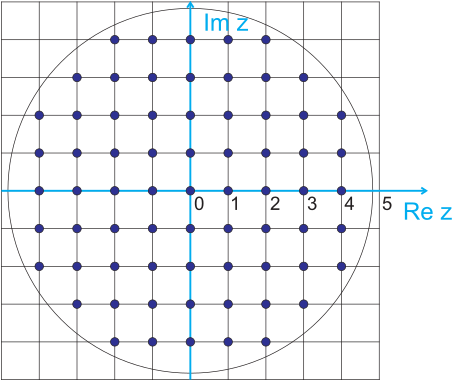
\includegraphics[width=6cm]{data/complex.png}
	\end{center}
	\begin{equation*}
		\begin{tabular}{|c|c|c|c|c|c||c|c|c|c|c|c|}\hline
			    & $z_k$ & $z_{k+1}$ & $a_{k+1}$ & $n:z_n=0$ & viz. &     & $z_k$ & $z_{k+1}$ & $a_{k+1}$ & $n:z_n=0$ & viz. \\ \hline \hline
			1.  & 0     &           &           & 0         &      & 36. & -3+2i & 3+i       & 1         & 9         & 30.  \\\hline
			2.  & 1     & 0         & 1         & 1         & 1.   & 37. & -3+i  & 2+i       & 0         & 4         & 14.  \\\hline
			3.  & i     & 1         & 1         & 2         & 2.   & 38. & -3-i  & 1+2i      & 0         & 7         & 15.  \\\hline
			4.  & -1+i  & 1         & 0         & 2         & 2.   & 39. & -3-2i & 1+3i      & 1         & 5         & 33.  \\\hline
			5.  & -i    & i         & 1         & 2         & 3.   & 40. & -2-3i & 3i        & 1         & 7         & 27.  \\\hline
			6.  & -1-i  & i         & 0         & 3         & 3.   & 41. & -1-3i & -1+2i     & 0         & 6         & 16.  \\\hline
			7.  & 1+i   & -i        & 0         & 3         & 5.   & 42. & 1-3i  & -2+i      & 0         & 5         & 17.  \\\hline
			8.  & -1    & 1+i       & 1         & 4         & 7.   & 43. & 2-3i  & -2+i      & 1         & 5         & 17.  \\\hline
			9.  & 1-i   & -1        & 0         & 5         & 8.   & 44. & 3-2i  & -2        & 1         & 5         & 12.  \\\hline
			10. & 2     & -1-i      & 0         & 4         & 6.   & 45. & 3-i   & -2-i      & 0         & 8         & 18.  \\\hline
			11. & 2i    & 1-i       & 0         & 6         & 9.   & 46. & 3+3i  & -3i       & 0         & 7         & 29.  \\\hline
			12. & -2    & 1+i       & 0         & 4         & 7.   & 47. & -3+3i & 3         & 0         & 5         & 26.  \\\hline
			13. & -2i   & -1+i      & 0         & 3         & 4.   & 48. & -3-3i & 3i        & 0         & 7         & 27.  \\\hline
			14. & 2+i   & -i        & 1         & 3         & 5.   & 49. & 3-3i  & -3        & 0         & 6         & 28.  \\\hline
			15. & 1+2i  & 1-i       & 1         & 6         & 9.   & 50. & 4     & -2-2i     & 0         & 8         & 24.  \\\hline
			16. & -1+2i & 2         & 1         & 5         & 10.  & 51. & 4i    & 2-2i      & 0         & 6         & 25.  \\\hline
			17. & -2+i  & 2+i       & 1         & 4         & 14.  & 52. & -4    & 2+2i      & 0         & 5         & 22.  \\\hline
			18. & -2-i  & 1+2i      & 1         & 7         & 15.  & 53. & -4i   & -2+2i     & 0         & 6         & 23.  \\\hline
			19. & -1-2i & 2i        & 1         & 7         & 11.  & 54. & 4+i   & -1-2i     & 1         & 8         & 19.  \\\hline
			20. & 1-2i  & -1+i      & 1         & 3         & 4.   & 55. & 4+2i  & -1-3i     & 0         & 7         & 41.  \\\hline
			21. & 2-i   & -1        & 1         & 5         & 8.   & 56. & 2+4i  & 1-3i      & 0         & 6         & 42.  \\\hline
			22. & 2+2i  & -2i       & 0         & 4         & 13.  & 57. & 1+4i  & 2-2i      & 1         & 6         & 25.  \\\hline
			23. & -2+2i & 2         & 0         & 5         & 10.  & 58. & -1+4i & 3-i       & 1         & 9         & 45.  \\\hline
			24. & -2-2i & 2i        & 0         & 7         & 11.  & 59. & -2+4i & 3-i       & 0         & 9         & 45.  \\\hline
			25. & 2-2i  & -2        & 0         & 5         & 12.  & 60. & -4+2i & 3+i       & 0         & 9         & 30.  \\\hline
			26. & 3     & -1-i      & 1         & 4         & 6.   & 61. & -4+i  & 3+2i      & 1         & 5         & 31.  \\\hline
			27. & 3i    & 2-i       & 1         & 6         & 21.  & 62. & -4-i  & 2+3i      & 1         & 5         & 32.  \\\hline
			28. & -3    & 2+2i      & 1         & 5         & 22.  & 63. & -4-2i & 1+3i      & 0         & 5         & 33.  \\\hline
			29. & -3i   & -1+2i     & 1         & 6         & 16.  & 64. & -2-4i & -1+3i     & 0         & 7         & 34.  \\\hline
			30. & 3+i   & -1-2i     & 0         & 8         & 19.  & 65. & -1-4i & -1+3i     & 1         & 7         & 34.  \\\hline
			31. & 3+2i  & -2i       & 1         & 4         & 13.  & 66. & 1-4i  & -2+2i     & 1         & 6         & 23.  \\\hline
			32. & 2+3i  & 1-2i      & 1         & 4         & 20.  & 67. & 2-4i  & -3+i      & 0         & 5         & 37.  \\\hline
			33. & 1+3i  & 1-2i      & 0         & 4         & 20.  & 68. & 4-2i  & -3-i      & 0         & 8         & 38.  \\\hline
			34. & -1+3i & 2-i       & 0         & 6         & 21.  & 69. & 4-i   & -2-i      & 1         & 8         & 18.  \\\hline
			35. & -2+3i & 3         & 1         & 5         & 26.  &     &       &           &           &           &      \\\hline
		\end{tabular}
	\end{equation*}\newpage
	Dokázali jsme, že existuje $k \in \mathbb{N}$ takové, že $z_{k+1} = 0$. Z toho plyne, že $z_k = a_k$,\newline odtud $z_{k-1} = a_k\cdot(-1+i)^1 + a_{k-1}$, \dots, $z = z_0 = a_k\cdot(-1+i)^k + a_{k-1}\cdot(-1+i)^{k-1} + \cdots + a_0$\newline Pokud zvolíme $a_j = 0$ pro $j > k$, pak $z=\sum_{j=0}^{\infty}a_j\cdot(-1+i)^j$
\end{proof}
\begin{remark} Algoritmus pro hledání reprezentace čísla v komplexní číselné soustavě
	\begin{enumerate}
		\item Nechť $z$ je číslo, které chceme reprezentovat, $z_0 = z$ a $j=0$ je počáteční hodnota algoritmu
		\item Provedeme následující operaci:\newline
		      $$x = \frac{(v_j-u_j)-(u_j+v_j)i}{2}$$
		      Jestliže $x \in \mathbb{Z}[i]$, pak $$z_{j+1} = x \quad a_{j+1}=0$$
		      V opačném případě $$z_{j+1} = \left\lceil\frac{(v_j-u_j)-(u_j+v_j)i}{2}\right\rceil\quad a_{j+1}=1$$
		\item Opakujeme operaci dokud $z_{j+1}\ne0$, nechť $n$ je počet iterací.\newline $(n$ je jistě konečné, viz. Důkaz \ref{kompDF}$)$
		\item $\{a_j\}_{j=0}^{\infty}$, kde $a_j=0$ pro každé $j>n$, splňuje požadavek $z=
			      \sum_{j=0}^{\infty}a_j\cdot(-1+i)^j$
	\end{enumerate}
\end{remark}
\subsection{Sčítání gaussových celých čísel v komplexní číselné soustavě}
Sčítání čísel v komplexní číselné soustavě můžeme provádět podle schématu popsaného v následujícím příkladu.
\begin{remark}
	Budeme postupovat obdobně jak u negabinární číselné soustavy.\newline Určíme si pravidla, která platí pro komplexní číselnou soustavu a následně nám ulehčí sčítání.\newline
	Pro lehčí orientaci v rovnostech si ukažme tabulku pár mocnin čísla $(-1+i)$ a zároveň se pro přehlednost domluvme,\newline že toto číslo budeme v některých případech po zbytek kapitoly značit $\beta$.
	\begin{equation}
		\begin{tabular}{|c|c|c|c|c|}
			\hline
			$\beta^0$ & $\beta^1 $ & $\beta^2$ & $\beta^3$ & $ \beta^4$ \\ \hline
			1         & -1+i       & -2i       & 2+2i      & -4         \\
			\hline
		\end{tabular}
	\end{equation}
	\newpage
	Protože $4\cdot\beta^k+\beta^{k+4}=4\cdot\beta^k+(-4)\cdot\beta^k=0$, platí následující:
	\begin{equation}\label{KompAddA}
		\begin{tabular}{|c|c|c|c|c|c|}
			\hline
			| & 0 & 0 & 0 & |||| & a+b \\ \hline
			0 & 0 & 0 & 0 & 0    & a+b \\
			\hline
		\end{tabular}
	\end{equation}
	Protože $2\cdot\beta^k+2\cdot\beta^{k+1}+\beta^{k+2}=2\cdot\beta^k+(-2+2i)\cdot\beta^k+(-2i)\beta^k=0$, platí následující:
	\begin{equation}\label{KompAddB}
		\begin{tabular}{|c|c|c|c|}
			\hline
			| & || & || & a+b \\ \hline
			0 & 0  & 0  & a+b \\
			\hline
		\end{tabular}
	\end{equation}
	Protože $2\cdot\beta^k-\beta^{k+2}-\beta^{k+3}=2\cdot\beta^k-(-2i)\cdot\beta^k-(2+2i)\cdot\beta^k=0$, platí následující:
	\begin{equation}\label{KompAddC}
		\begin{tabular}{|c|c|c|c|c|}
			\hline
			0 & 0 & 0 & || & a+b \\ \hline
			| & | & 0 & 0  & a+b \\
			\hline
		\end{tabular}
	\end{equation}
\end{remark}
\begin{example}
	\item Zvolme $a = 4+3i$ a $b = 3-4i$. Dle výše uvedeného algoritmu nalezneme ciferný zápis těchto gaussových celých čísel: $4+3i = (1100111)_{(-1+i)}$ a $3-4i = (111101)_{(-1+i)}$. Cifry zapíšeme pod sebe do tabulky a do řádku pod nimi naznačíme pomocí čárek, kolik má součet $a+b$ příslušných mocnin čísla $(-1+i)$:
	\begin{equation}\label{KompAddT1}
		\begin{tabular}{|c|c|c|c|c|c|c|c|}
			\hline
			1 & 1  & 0 & 0 & 1  & 1 & 1  & a   \\ \hline
			0 & 1  & 1 & 1 & 1  & 0 & 1  & b   \\ \hline \hline
			| & || & | & | & || & | & || & a+b \\
			\hline
		\end{tabular}
	\end{equation}
	Vzhledem k (\ref{KompAddA}), (\ref{KompAddB}) a (\ref{KompAddC}) můžeme v úpravách Tabulky (\ref{KompAddT1}) pokračovat následujícím způsobem:
	\begin{equation}\label{KompAddT2}
		\begin{tabular}{|c|c|c|c|c|c|c|c|c|c|c|}
			\hline
			0             & 0             & 1 & 1              & 0             & 0              & 1               & 1 & 1              & a   &                  \\ \hline
			0             & 0             & 0 & 1              & 1             & 1              & 1               & 0 & 1              & b   &                  \\ \hline \hline
			0             & 0             & | & ||             & |             & \underline{|}  & \underline{||}  & | & \underline{||} & a+b & (\ref{KompAddC}) \\
			0             & 0             & | & ||             & \underline{|} & \underline{||} & \underline{|||} & | & 0              & a+b & (\ref{KompAddB}) \\
			\underline{0} & \underline{0} & | & \underline{||} & 0             & 0              & |               & | & 0              & a+b & (\ref{KompAddB}) \\
			|             & |             & | & 0              & 0             & 0              & |               & | & 0              & a+b &                  \\
			\hline
		\end{tabular}
	\end{equation}
	Z posledního řádku vyčteme, že $a + b = (111000110)_{(-1+i)}$\newline A opravdu, $\beta^8+\beta^7+\beta^6+\beta^2+\beta^1=16-8-8i+8i-2i-1+i=\underline{7-i}=4+3i+3-4i$
\end{example}
\newpage
\subsection{Nalezení opačného čísla v komplexní číselné soustavě}

K danému číslu $z$ hledáme číslo opačné. Když se zamyslíme jak součtem různých mocnin čísla $(-1+i)$ dojít k výsledku $-1$, po chvíli dojedme k následujícímu:
$$\beta^0+\beta^1+\beta^1+\beta^2=1+(-1+i)+(-1+i)+(-2i)=-1$$
Uvědomme si, že násobení mocninou čísla $(-1+i)^k, k\in\mathbb{N}_0$ znamená posunutí všech cifer o $k$ míst (doleva) a připsání $k$ nul na konec ciferného zápisu. Umíme-li už gaussova celá čísla sčítat, pak nalezení čísla opačného už nebude takový problém. Uvedeme příklad.
\begin{example}
	Nalezneme číslo opačné k číslu $z = -1+2i = (11001)_{(-1+i)}$
	\begin{equation}\label{KompSoucA}
		\begin{tabular}{|c|c|c|c|c|c|c|c|}
			\hline
			0             & 0               & 1               & 1             & 0              & 0              & 1 & $z$              \\ \hline
			0             & 1               & 1               & 0             & 0              & 1              & 0 & $\beta\cdot z$   \\ \hline
			0             & 1               & 1               & 0             & 0              & 1              & 0 & $\beta\cdot z$   \\ \hline
			1             & 1               & 0               & 0             & 1              & 0              & 0 & $\beta^2\cdot z$ \\ \hline \hline
			\underline{|} & \underline{|||} & \underline{|||} & \underline{|} & \underline{|}  & \underline{||} & | & $-z$             \\\hline
			0             & \underline{|}   & \underline{|}   & 0             & \underline{-|} & 0              & | & $-z$             \\
			\hline
			0             & 0               & 0               & 0             & |              & 0              & | & $-z$             \\
			\hline
		\end{tabular}
	\end{equation}
	Proto $-z = (101)_{(-1+i)}$. A opravdu, $\beta^0 + \beta^2 = \underline{1-2i} = -(z)=-(-1+2i)$
\end{example}
\begin{remark}
	Jistě některé z čtenářů napadne otázka, zda-li by nějak jednoduše šlo najít\newline k gaussovu celému číslu jeho číslo komplexně sdružené v reprezentaci komplexní číselné soustavy.\newline Bez převádění do desítkové soustavy a zpět bychom se však při takovém pokusu bohužel neobešli. Uvědomíme-li si, že na rozdíl od hledání opačného čísla, kde stačí číslo vynásobit číslem $-1$,\newline u hledání komplexně sdruženého čísla je proces těžší. Číslo $x$, kterým bychom naše\newline gaussovo celé číslo $z$ museli přenásobit je závisle právě na téže číslu ($z$). Nelze najít obecnou formuli jako v případě hledání opačného čísla (např: "vynásob číslo číslem $-1$").
\end{remark}\newpage
\subsection{Násobení v komplexní číselné soustavě}
Násobení v komplexní soustavě je analogické násobení v desítkové soustavě. Násobíme-li číslo $a = (a_n, \dots, a_0)_{(-1+i)}$ číslem $(-1+i)^k = (1, \underbrace{0, \dots, 0}_{k\text{ nul}})_{(-1+i)}$, pak stačí přidat na konec ciferného zápisu $k$ nul:
$$(1, \underbrace{0, \dots, 0}_{k\text{ nul}})_{(-1+i)}\cdot(a_n, \dots, a_0)_{(-1+i)} = (a_n, \dots, a_0, \underbrace{0, \dots, 0}_{k\text{ nul}})_{(-1+i)}$$
Proto pro součin čísel $a = (a_n, \dots, a_0)_{(-1+i)}$ a $b = (b_k, \dots, b_0)_{(-1+i)}$ platí
\begin{equation}\label{complexMultiplication}
	a\cdot b = \sum_{i=0}^{k} a_i\cdot(b_k, \dots, b_0, \underbrace{0, \dots, 0}_{i\text{ nul}} )_{(-1+i)}
\end{equation}
Demonstrujeme na příkladu
\begin{example}
	Vynásobíme čísla $a = (4-i) = (111010111)_{(-1+i)}$ a $b = (1-2i) = (101)_{(-1+i)}$\newline
	\begin{center}
		\begin{tabular}{ccccccccccccc}
			        &   &   & 1 & 1 & 1 & 0 & 1                   & 0 & 1 & 1 & 1 & ( = a )     \\
			$\cdot$ &   &   &   &   &   &   &                     &   & 1 & 0 & 1 & ( = b )     \\ \hline
			        &   &   & 1 & 1 & 1 & 0 & 1                   & 0 & 1 & 1 & 1 & ( = $x_1$ ) \\
			+       &   &   &   &   &   &   &                     &   &   & 0 &   & ( = $x_2$ ) \\
			+       & 1 & 1 & 1 & 0 & 1 & 0 & 1                   & 1 & 1 &   &   & ( = $x_3$ ) \\&&&&&&&&&&&&\\
			        &   &   &   &   &   &   & $\Leftrightarrow\;$ &   &   &   &   &             \\
		\end{tabular}
	\end{center}
	$$ (111010111)_{(-1+i)} \cdot(101)_{(-1+i)} $$$$=$$$$ 1\cdot(111010111)_{(-1+i)} + 0 \cdot(1110101110)_{(-1+i)} + 1\cdot (11101011100)_{(-1+i)} $$$$=$$$$ (111010111)_{(-1+i)} + (11101011100)_{(-1+i)}$$\newpage
	Můžeme sečíst schematicky:
	\begin{equation}
		\begin{tabular}{|c|c|c|c|c|c|c|c|c|c|c|c|}
			\hline
			0             & 0              & 1               & 1             & 1              & 0             & 1               & 0 & 1              & 1 & 1 & $x_1$       \\ \hline
			1             & 1              & 1               & 0             & 1              & 0             & 1               & 1 & 1              & 0 & 0 & $x_3$       \\ \hline \hline
			|             & \underline{|}  & \underline{|}|  & |             & \underline{||} & \underline{0} & \underline{||}  & | & \underline{||} & | & | & $x_1 + x_3$ \\ \hline
			|             & ||             & \underline{|||} & |             & 0              & |             & \underline{|||} & | & 0              & | & | & $x_1 + x_3$ \\ \hline
			\underline{|} & \underline{||} & \underline{||}  & |             & 0              & |             & -|              & | & 0              & | & | & $x_1 + x_3$ \\ \hline
			0             & 0              & 0               & \underline{|} & \underline{0}  & |             & \underline{-|}  & | & 0              & | & | & $x_1 + x_3$ \\ \hline
			0             & \underline{0}  & \underline{0}   & 0             & \underline{-|} & |             & |               & | & 0              & | & | & $x_1 + x_3$ \\ \hline
			0             & \underline{-|} & \underline{-|}  & 0             & |              & |             & |               & | & 0              & | & | & $x_1 + x_3$ \\ \hline
			|             & |              & |               & 0             & |              & |             & |               & | & 0              & | & | & $x_1 + x_3$ \\ \hline
		\end{tabular}
	\end{equation}
	Výpočtem ověřme.\newline $(11101111011)_{(-1+i)}=(-32i)+(-16+16i)+(16)+(8i)+(4-4i)+(-4)+(2+2i)+(-1+i)+(1)=\underline{2-9i}=4-2-i-8i=(4-i)\cdot(1-2i)=a\cdot b$\newline Výsledek je správně.
\end{example}
\subsection{Výhody a nevýhody komplexní číselné soustavy}
V tomto případě jde o zvláštní číselnou soustavu, která umožňuje reprezentovat libovolné gaussovo celé číslo jako posloupnost jedniček a nul. V praxi bychom této skutečnosti mohli využít například při kódování analogového signálu pomocí QAM \cite{giApplic}. Nevýhody neshledávám žádné.
\section{Negafibonacciho číselná soustava}
\begin{definition}
	Negafibonacciho číselná soustava je číselná soustava na okruhu $(\mathbb{Z},+,\cdot)$ o základu $\poslalpha = \{F_{-(i+1)}\}_{i=0}^{\infty}$ (kde $F_{-i}$ je i-tý člen Negafibonacciho posloupnosti)\newline s množinou cifer $C=\{0,1\}$
\end{definition}
\begin{remark}
	Nenechme se zmást symbolem \textbf{'$-$'} u indexu členu Negafibonacciho posloupnosti. Používá se pro odlišení od členů Fibonacciho posloupnosti. Nejde však o záporný index!\newline Proto pro přehlednost můžeme psát indexy (např. $(i+1)$) do závorky.
\end{remark}
\begin{definition}\label{fiboDef} \textbf{Negafibonacciho posloupnost}\newline
	Je nekonečná posloupnost přirozených čísel definována rekurentní formulí:
	$$F_{-0} = 0,\quad F_{-1} = 1,\quad F_{-n} = F_{-(n-2)} - F_{-(n-1)}$$
\end{definition}
Z Definice \ref{fiboDef} si lehce rozmyslíme, že každý další člen bude střídavě záporný kladný\newline a jeho absolutní hodnota bude větší než u předchozích členů.\newline
Negafibonacciho posloupnost je velice podobná Fibonacciho posloupnosti.
$$F_{-n} = (-1)^{n+1}\cdot F_n$$
\begin{example}
	$$F_{-2} = F_{-0} - F_{-1} = 0 - 1 = -1$$$$F_{-3 }= F_{-1}-F_{-2} = 1-(-1)=2$$$$F_{-4} = F_{-2} - F_{-3} = -1 -2 = -3$$$$\vdots$$
	$$ \{F_{-(i+1)}\}_{i=0}^{\infty} = \{1,-1,2,-3,5,-8,13,-21,34,-55,89,\dots\}$$
\end{example}
\begin{agreement}
	V Negafibonacciho číselné soustavě zapisujeme:
	$\varphi(x) = (\posla)_F$\newline
\end{agreement}
\begin{remark}
	Podle definice se jedná o nejednoznačnou číselnou soustavu, což si ukážeme\newline v následujícím příkladu.
\end{remark}\newpage
\begin{example}
	Každé číslo, vezměme si například $27$, můžeme zapsat více způsoby (nekonečně mnoha).\newline
	\begin{center}\begin{tabular}{c c c c c}
			$27$ & = & $34-8+1$         & = & $ (100100001)_F$     \\
			     & = & $34-21+13+1$     & = & $ (111000001)_F$     \\
			     & = & $89-55-8+1$      & = & $ (11000100001)_F$   \\
			     & = & $233-144-55-8+1$ & = & $ (1101000100001)_F$ \\
		\end{tabular}\end{center}
\end{example}
\begin{theorem}
	Analogie Zeckendorfovy věty pro Fibonacciho kódování. \cite{fibCoding}\newline
	Pro každé celé číslo $z$ existuje posloupnost $\posla$ splňující podmínky:
	\begin{itemize}
		\item $z=\sum_{i=0}^{\infty}a_i\cdot F_{-(i+1)}$, ( důsledkem je, že $D(\varphi) = \mathbb{Z}$ )
		\item $a_k\cdot a_{k+1}=0$ ( tj. v posloupnosti nejsou nikdy dvě jedničky vedle sebe)
	\end{itemize}
\end{theorem}
\begin{proof}\label{fiboDF}
	Buď libovolné $z\in\mathbb{Z}$ dáno. Rozdělme si jej na případy.
	\begin{itemize}
		\item $z=0$ V tomhle případě klademe každý člen posloupnosti $a_i = 0$
		\item $z<0$ Označme $n \in \mathbb{N}$ nejmenší index, pro který platí $z>-F_{-n}$ a položme $a_{n-2}=1$\newline ( poznámka : $(n-2)$ namísto $(n-1)$, protože základ je posunut $\{F_{-(i+1)}\}_{i=0}^{\infty}$,\newline zároveň díky podmínce $z<0$ nebude index nikdy záporný ). Takový index jistě najdeme, protože z Negafibonacciho posloupnosti lze vybrat posloupnost vybranou, která je\newline nekonečná a klesající. Nyní uvažujme o čísle $z_{1} = -F_{-(n-1)}+z$.
		      Uvědomme si,\newline že $F_{-(n-1)}$ je záporné, protože $F_{-n}$ je kladné ( $z>-F_{-n}$ ). Zároveň víme,\newline že $-F_{-(n-1)}$ je menší než $-2z$. Jak toto víme? Dokážeme sporem. Předpokládejme, že
		      $$-F_{-(n-1)} \ge -2z$$
		      $$F_{-(n-1)} \le 2z < z$$Poslední nerovnost platí díky tomu, že $z < 0$
		      $$-F_{-(n-2)}\le\frac{F_{-(n-1)}}{2}\le z$$
		      Zde vidíme, že by existovalo $(n-2)$, pro které platí $z>-F_{-(n-2)}$, což je v rozporu\newline s minimalitou $n$.\newline Když víme, že $-F_{-(n-1)}$ je menší než $-2z$, pak jistě bude platit $|z_1|<|z|$.\newline S číslem $z_1$ provedeme znova stejnou úvahu, kde dvojice $z_1,z_2$ vystřídá dvojici $z, z_1$.\newline Posloupnost čísel $z_{k}$ se v konečném počtu kroků předchozích úvah dostane k nule.\newline V případě, že nějaké $z_i > 0$, se pomocí vysvětlivek v $z>0$ taky v následujícím kroku přiblížíme nule.
		\item $z>0$ Označme $n \in \mathbb{N}$ nejmenší index, pro který platí $z\le-F_{-n}$ a položme $a_{n-2}=1$\newline ($(n-2)$ můžeme použít jako index, protože díky podmínce $z>0$ nebude nikdy záporný )\newline Takový index jistě najdeme, protože z Negafibonacciho posloupnosti lze vybrat posloupnost vybranou, která je nekonečná a roustoucí. Nyní uvažujme o čísle $z_{1} = -F_{-(n-1)}+z$.
		      Uvědomme si, že $F_{-(n-1)}$ je kladné, protože $F_{-n}$ je záporné ( $z\le-F_{-n}$ ). Zároveň víme, že $-F_{-(n-1)}$ je větší než $-2z$. Jak toto víme? Dokážeme sporem. Předpokládejme, že
		      $$-F_{-(n-1)} \le -2z$$
		      $$F_{-(n-1)} \ge 2z$$
		      $$-F_{-(n-2)}\ge\frac{F_{-(n-1)}}{2}\ge z$$
		      Zde vidíme, že by existovalo $(n-2)$, pro které platí $z\le-F_{-(n-2)}$, což je v rozporu s minimalitou $n$. Když víme, že $-F_{-(n-1)}$ je větší než $-2z$, pak jistě bude platit $|z_1|<|z|$
	\end{itemize}
	Jestliže je číslo nenulové, pak klademe $a_i=0$ pro $i>n-2$,\newline kde $n$ je zprvu zvolený nejmenší index. \newline
	$\posla$ je posloupnost s konečným počtem nenulových členu, proto platí\newline $z=\sum_{i=0}^{k_0}a_i\cdot F_{-(i+1)}$, kde $z_{k_0}=0$\newline
	Takto zkonstruována posloupnost $\posla$ nebude mít nikdy dvě jedničky vedle sebe.\newline V případě kdyby vedle sebe byly, pak jsme volili špatně nejmenší $n$.
\end{proof}
\begin{remark}\label{compAlg} Algoritmus pro hledání reprezentace čísla v negafibonacciho číselné soustavě
	\begin{enumerate}
		\item Nechť $z$ je číslo, které chceme reprezentovat, $z_0 = z$ a $k=0$ jsou počáteční hodnoty algoritmu.
		\item Jestliže je $z_0=0$, algoritmus ukončíme a zapíšeme $a_i=0$
		\item V případě, že $z_k$ je kladné, pak najdeme nejmenší $n$ pro které platí $z_k\le-F_{-n}$\newline v případě, že je záporné hledáme nejmenší $n$, pro které platí $z_k>-F_{-n}$
		\item Zapíšeme si na pozici $a_{n-2} = 1$
		\item Spočítáme si $z_{k+1} = -F_{-(n-1)}+z_k$\newline Jestliže je $z_{k+1}=0$, pak pro ostatní pozice posloupnosti zapíšeme $a_i=0$,\newline kde $i>0$ a $i<(n-2)$
		\item V případě, že $z_{k+1}\ne 0$, algoritmus opakujeme.
	\end{enumerate}
\end{remark}\newpage
\subsection{Sčítání celých čísel v negafibonacciho číselné soustavě}
Sčítání čísel v negafibonacciho číselné soustavě můžeme provádět podle schématu popsaného\newline v následujícím příkladu.
\begin{remark}
	Následující rovnosti nám pomůžou v sčítání čísel v negafibonacciho číselné\newline soustavě.
	Protože $F_{-k}-F_{-(k+1)}-F_{-(k+2)}=0$ (z Definice \ref{fiboDef}), platí následující:
	\begin{equation}\label{fiboAddA}
		\begin{tabular}{|c|c|c|c|c|c|}
			\hline
			| & | & 0 & a+b \\ \hline
			0 & 0 & | & a+b \\
			\hline
		\end{tabular}
	\end{equation}
	Protože $$\underline{F_{-(k+3)}-2\cdot F_{-(k+1)}+F_{-k}}=-F_{-(k+2)}+F_{-(k+1)}-2\cdot F_{-(k+1)}+F_{-k}=-F_{-(k+2)}-F_{-(k+1)}+F_{-k}=0$$platí následující:
	\begin{equation}\label{fiboAddB}
		\begin{tabular}{|c|c|c|c|c|}
			\hline
			0 & 0 & || & 0 & a+b \\ \hline
			| & 0 & 0  & | & a+b \\
			\hline
		\end{tabular}
	\end{equation}
	Protože $$\underline{-F_{-(k+4)}+3\cdot F_{-(k+2)}-F_{-k}}=F_{-(k+3)}-F_{-(k+2)}+3\cdot F_{-(k+2)}-F_{-k}=$$$$=\underline{F_{-(k+3)}+2\cdot F_{-(k+2)}-F_{-k}}=$$$$=2\cdot F_{-(k+2)}-F_{-(k+2)}+F_{-(k+1)}-F_{-k}=F_{-(k+2)}+F_{-(k+1)}-F_{-k}=0$$platí následující:
	\begin{equation}\label{fiboAddC}
		\begin{tabular}{ccc}
			\begin{tabular}{|c|c|c|c|c|c|}
				\hline
				0 & 0 & ||| & 0 & 0 & a+b \\ \hline
				| & 0 & 0   & 0 & | & a+b \\
				\hline
			\end{tabular}
			 & a &
			\begin{tabular}{|c|c|c|c|c|}
				\hline
				| & || & 0 & 0 & a+b \\ \hline
				0 & 0  & 0 & | & a+b \\
				\hline
			\end{tabular}
		\end{tabular}
	\end{equation}
\end{remark}
\begin{example}
	\item Zvolme například $a = 17$ a $b = 23$. Dle výše uvedeného algoritmu nalezneme ciferný zápis těchto celých čísel $17 = (1010010)_F$ a $23 = (100101000)_F$
	\begin{equation}\label{fiboAddT1}
		\begin{tabular}{|c|c|c|c|c|c|c|c|c|c|}
			\hline
			  &   & 1 & 0 & 1 & 0 & 0 & 1 & 0 & a   \\ \hline
			1 & 0 & 0 & 1 & 0 & 1 & 0 & 0 & 0 & b   \\ \hline \hline
			| & 0 & | & | & | & | & 0 & | & 0 & a+b \\
			\hline
		\end{tabular}
	\end{equation}
	\newpage
	Vzhledem k (\ref{fiboAddA}), (\ref{fiboAddB}) a (\ref{fiboAddC}) můžeme v úpravách Tabulky (\ref{fiboAddT1}) pokračovat následujícím způsobem:
	\begin{equation}\label{fiboAddT2}
		\begin{tabular}{|c|c|c|c|c|c|c|c|c|c|c|}
			\hline
			              &   & 1               & 0             & 1             & 0             & 0             & 1             & 0 & a   &                  \\ \hline
			1             & 0 & 0               & 1             & 0             & 1             & 0             & 0             & 0 & b   &                  \\ \hline \hline
			|             & 0 & |               & |             & \underline{|} & \underline{|} & 0             & |             & 0 & a+b & (\ref{fiboAddA}) \\
			\underline{|} & 0 & \underline{|}   & \underline{|} & 0             & 0             & |             & |             & 0 & a+b & (\ref{fiboAddB}) \\
			0             & 0 & |||             & 0             & 0             & 0             & \underline{|} & \underline{|} & 0 & a+b & (\ref{fiboAddA}) \\
			0             & 0 & \underline{|||} & 0             & 0             & 0             & 0             & 0             & | & a+b & (\ref{fiboAddC}) \\
			|             & 0 & 0               & 0             & |             & 0             & 0             & 0             & | & a+b & (\ref{fiboAddC}) \\
			\hline
		\end{tabular}
	\end{equation}
	Z posledního řádku vyčteme, že $a + b = (100010001)_F$\newline A skutečně, $F_{-9}+F_{-5}+F_{-1}=34+5+1=\underline{40}=17+23$
\end{example}
\begin{remark}
	Kvůli charakteru této soustavy nemůžeme hovořit o hledání opačného čísla ani o násobení čísel. V některých případech bychom se k opačnému číslu dobrali, ale postup nelze generalizovat a najít číslo vždy.\newline
	Například si ukážeme jak najít číslo opačné pro číslo $6 = (10001)_F$
	\begin{equation}
		\begin{tabular}{|c|c|c|c|c|c|c|c|}
			\hline
			  & 1              & 0             & 0 & 0               & 1              & a  &                                            \\ \hline
			  & -|             & 0             & 0 & 0               & \underline{-|} & -a & (\ref{fiboAddB})                           \\
			  & \underline{-|} & \underline{|} & 0 & -||             & 0              & -a & (\ref{fiboAddA})                           \\
			| & 0              & 0             & 0 & \underline{-||} & 0              & -a & $-2\cdot F_{-2} = -2\cdot-1 = 2 = F_{-3} $ \\
			| & 0              & 0             & | & 0               & 0              & -a & $-2\cdot F_{-2} = -2\cdot-1 = 2 = F_{-3} $ \\
			\hline
		\end{tabular}
	\end{equation}
	a opravdu $F_{-6}+F_{-3}=-8+2=-6=(100100)_F$
\end{remark}
\subsection{Výhody a nevýhody negafibonacciho číselné soustavy}
Tato číselná soustava je vlastně rozšířením definičního oboru Fibonacciho kódování \cite{fibCoding} na obor celých čísel. Proto má stejné výhody. Pokud reprezentujeme číslo způsobem popsaným\newline v Poznámce \ref{compAlg}, pak nebude mít dvě jedničky vedle sebe. Toho se dá využít při komunikaci dvou zařízení, kdy se oba nastaví tak, že každá n-tice znaků bude oddělena dvěmi jedničkami.\newline S tímhle přístupem je pak mnohem jednodušší odhalit chybu při přenosu, která se projeví například tím, že mezi oddělovači (dvě jedničky) nebude n znaků. Znaky může být binární signál, a proto by tento přístup byl vhodný pro přenášení digitálních dat. Kromě toho je výhodou definiční obor. Není třeba definovat jakým způsobem se při přenosu označí záporné číslo.

\section{Faktoriálová číselná soustava}
\begin{definition}
	Faktoriálová číselná soustava je číselná soustava na okruhu $(\mathbb{Z},+,\cdot)$ o základu $\poslalpha = \{(i+1)!\}_{i=0}^\infty$ s množinou cifer $C=\mathbb{N}_0$
\end{definition}
\begin{remark}
	Možná Vás jako čtenáře překvapila množina cifer, a skutečně se nejedná o žert. Cílem této práce však není najít nejefektivnější řešení, ale prozkoumat teoretické možnosti.\newline Je jasné, že neexistuje dostatek unikátních znaků pro pokrytí celé množiny $\mathbb{N}_0$, proto je tato\newline soustava více teoretická a neuveditelná do praxe. Pro splnění cíle této práce si postačíme s její konečnou podmnožinou.
\end{remark}
\begin{agreement}
	Nechť ve zbytku kapitoly symboly $A = 10, B = 11, C = 12, ... Z = 35$ označují příslušnou cifru.
\end{agreement}
\begin{agreement}
	V faktoriálové číselné soustavě zapisujeme:
	$\varphi(x) = (\posla)_!$\newline
	Hledáme-li relaci k zápornému číslu, pak podobně jak jsme zvyklí v desítkové číselné soustavě, najdeme reprezentaci čísla opačného a zapíšeme znaménko \textbf{`$-$`} před reprezentaci.
\end{agreement}
\begin{remark}
	Je dobré si uvědomit, že se nejedná o jednoznačnou číselnou soustavu.\newline Předveďme si pár způsobů jak reprezentovat číslo $10$.
	\begin{center}
		\begin{tabular}{c c c c c}
			$10$ & = & $10\cdot1$        & = & $(A)_!$   \\
			     &   & $5\cdot2$         & = & $(50)_!$  \\
			     &   & $1\cdot6+2\cdot2$ & = & $(120)_!$ \\
			     &   & \vdots            &   &
		\end{tabular}
	\end{center}
\end{remark}
\begin{theorem}
	Pro každé $x \in \mathbb{N}_0$ existuje posloupnost $\posla: x=
		\sum_{i=0}^{\infty}a_i\cdot (i+1)_!$\newline To jest $D(\varphi)=\mathbb{N}_0$
\end{theorem}
\begin{proof}\label{faktDF}
	Nechť $x\in\mathbb{Z}$ je dáno. Jestliže je $x=0$, pak je v relaci s $(0)_!$ V případě, že $x\ne0$ hledejme největší $n\in\mathbb{N}$, pro které platí: $n!\le x$. Takové jistě najdeme, protože posloupnost $\{(i+1)!\}_{i=0}^\infty$ je rostoucí a nekonečná. Následně si zapíšeme $a_{n-1}=\left\lfloor\frac{x}{n!}\right\rfloor$ (protože základ soustavy je posunut). Jelikož je $x\ge n!$, bude $a_{n-1}$ jistě rovno alespoň $1$. Následně uvažujme $x_1 = x - a_{n-1}\cdot n!$\newline (což je v podstatě zbytek po celočíselném dělení).
	Protože je $x_1$ zbytek po dělení čísla x číslem $n!$, platí $x_1<n!\le x$. Stejnou úvahu provádíme dokud nedostaneme $x_k=0$. Místo původního čísla $x$ dosazujeme $x_k$. Obdržíme další cifru $a_i$ a celé číslo $x_{k+1}<x_k$. Po konečném kroku se dostaneme k $x_k=0$. Všechny členy posloupnosti, které nebyly určeny položíme $a_i=0$\newline včetně těch, kde $i\ge n$ a $n$ volíme zprvu zvolené. Pro takto vytvořenou posloupnost platí: $$x=\sum_{i=0}^\infty a_i\cdot(i + 1)!$$\newpage
\end{proof}
\begin{remark}\label{algoFakt} Algoritmus pro hledání reprezentace čísla v faktoriálové číselné soustavě
	\begin{enumerate}
		\item Nechť $x$ je číslo, které chceme reprezentovat, $x_0 = x$ a $i=0$ je počáteční hodnota algoritmu
		\item Najdeme nejvyšší n, pro které platí: $n! < x$
		\item Provedeme následující operaci:\newline $x_i/(n-i)!=a_{n-i-1}\;zb.\;x_{i+1}$, kde $ a_i,x_i\in\mathbb{N}_0$
		\item Opakujeme operaci, s tím, že k $i$ přičteme $1$, dokud $x_{i+1}\ne0$.
	\end{enumerate}
\end{remark}
\begin{example}
	$$z=77$$
	$$77:4!=3\,zb.\,5$$
	$$5:3!=0\,zb.\,5$$
	$$5:2!=2\,zb.\,1$$
	$$1:1!=1\,zb.\,0$$
	$$\Rightarrow a_0=1, a_1=2,a_2=0,a_3=3$$
	$$ 77 = 1 \cdot 1! + 2 \cdot 2! + 3\cdot 4!$$
	$$ 77 = 1 + 4 + 72 \quad \checkmark$$
\end{example}
\subsection{Sčítání celých čísel v faktoriálové číselné soustavě}
Sčítání čísel v faktoriálové číselné soustavě můžeme provádět podle schématu popsaného\newline v následujícím příkladu.
\begin{remark}
	Sčítání čísel provádíme velice podobně jak jsme zvyklí v desítkové soustavě,\newline tj. sepíšeme si čísla po sebe a sčítáme po řádech. Jediný rozdíl je pravidlo pro přenesení přebytku na vyšší řád. U desítkové soustavy máme $10$ cifer a jsme zvyklí při součtu větším než $9$ přenést $1$ na vyšší řád a zapsat zbytek po odečtení $10$ od součtu. U této soustavy bude tato hranice pro přenesení záviset na indexu s kterým právě počítáme.
	Např. u indexu $3$, kde $a_3\in\{0,1,2,3\}$ budeme přenášet při překročení čísla $3$, tj. $4$ a více. Toto pravidlo je zřejmé z definice faktoriálu$$3!\cdot4=4!$$
\end{remark}
\begin{example}
	\item Zvolme například $a = 63$ a $b = 91$. Dle algoritmu popsaného v Poznámce \ref{algoFakt} nalezneme ciferný zápis těchto celých čísel: $63 = (2211)_!$ a $91 = (3301)_!$
	\begin{equation}\label{faktAddT1}
		\begin{tabular}{|c|c|c|c|c|c|}
			\hline
			 & 2      & 2             & 1      & 1             & a                     \\ \hline
			 & 3      & 3             & 0      & 1             & b                     \\ \hline \hline
			 & $\ge5$ & $\ge4$        & $\ge3$ & $\ge2$        & hranice pro přenesení \\ \hline
			 & 5      & 5             & 1      & \underline{2} & a+b                   \\ \hline
			 & 5      & \underline{5} & 2      & 0             & a+b                   \\ \hline & \underline{6} & 1             & 2      & 0             & a+b                   \\ \hline 1 & 1             & 1             & 2      & 0             & a+b                   \\ \hline
		\end{tabular} \end{equation} Z posledního řádku vyčteme, že $a + b = (11120)_!$\newline A skutečně, $1\cdot5!+1\cdot4!+1\cdot3!+2\cdot2!=120+24+6+4=\underline{154}=63+91$
\end{example}
\subsection{Výhody a nevýhody faktoriálové číselné soustavy} Tato číselná soustava nemá žádné výhody co se týče použitelnosti. Hlavním problémem je, jak jsme zmínili v úvodu, rostoucí potřeba pro cifry při převodu větších čísel. Postrádá oproti předchozím soustavám výhodu reprezentace záporných čísel bez pomocných symbolů.\newline Co ale této soustavě nemůžeme upřít je její jednoduchost, hezké využití faktoriálu,\newline příjemné sčítání. V praxi se tedy dá použít jedině pro výuku.
\section{Závěr}
Všechny čtyři číselné soustavy jsme prozkoumali, některé podrobněji, a některé méně.\newline Hlavním cílem u dokazování definičního oboru číselné soustavy je ukázka toho, že algoritmus vždy po nějakém počtu kroků dosáhne svého cíle, a to nuly. Sčítání a násobení je u těchto\newline pozičních soustav obdobné jak u desítkové soustavy, kterou všichni dobře znají. Jen je třeba si určit nějaké pravidla, která nám při operacích pomohou.\newline\newline Zajimavým zjištěním byl fakt, že oproti standardním číselným soustavám, kde je základem\newline nějaké přirozené číslo, u nestandardních (konkrétně u komplexní) si jako základ nemůžeme\newline vybrat libovolné číslo (samozřejmě víme, že čím menší norma čísla, tím je menší množina\newline potřebných znaků pro reprezentaci celého definičního oboru). Takovým příkladem byla\newline komplexní soustava. Při pokusech jsme zjistili, že v číselné soustavě\newline se základem $(1-i)$ a $C=\{0,1\}$ nenajdeme reprezentaci pro všechna gaussova celá čísla,\newline i přesto, že norma základu je stejná jako norma základu s kterým jsme definiční obor dokázali $(-1+i)$.\newline\newline Tématem, kterým jsme se v této práci nezabývali a bylo by záhodno ji o něj doplnit, je rozšíření již popsaných číselných soustav na číselné soustavy na tělese (to jsou ty,\newline které umožňují reprezentovat čísla z množiny reálných čísel). Dalším velice zajimavým typem číselných soustav jsou číselné soustavy s iracionálním základem ($e$, $\sqrt{2}$, $\varphi$).
\printbibliography[title={Literatura}, heading=bibintoc]
\end{document}
